%%%%%%%%%%%%%%%%%%%%%%%%%%%%%%%%%%%%%%%%%
% Beamer Presentation
% LaTeX Template
% Version 1.0 (10/11/12)
%
% License:
% CC BY-NC-SA 3.0 (http://creativecommons.org/licenses/by-nc-sa/3.0/)
%
%%%%%%%%%%%%%%%%%%%%%%%%%%%%%%%%%%%%%%%%%

%----------------------------------------------------------------------------------------
%	PACKAGES AND THEMES
%----------------------------------------------------------------------------------------

\documentclass[usenames,dvipsnames]{beamer}

\newcommand{\magicsectionpage}[1]{\begin{frame}
\vfill
\centering
\begin{beamercolorbox}[sep=8pt,center,shadow=true,rounded=true]{title}
\usebeamerfont{title}#1\par
\end{beamercolorbox}
\vfill
\end{frame}
}

%\usepackage[dvipsnames]{xcolor}
\definecolor{grey}{gray}{0.3}
\definecolor{STFCBlue}{HTML}{2E2D62}

\usetheme{Madrid}
\useoutertheme{infolines} % Alternatively: miniframes, infolines, split
\useinnertheme{rounded}
\setbeamertemplate{footline}[frame number] % To replace the footer line in all slides with a simple slide count uncomment this line
\setbeamertemplate{navigation symbols}{} % To remove the navigation symbols from the bottom of all slides uncomment this line

\setbeamersize{text margin left=3em, text margin right=3em}


\setbeamercolor{title}{fg=white, bg=STFCBlue}
\setbeamercolor{titlelike}{fg=white}
\setbeamercolor{frametitle}{fg=white}

\setbeamercolor{normal text}{fg=black}
\setbeamercolor{separation line}{}
\setbeamercolor{sidebar}{bg=STFCBlue}
\setbeamercolor{section in sidebar}{fg=white}
\setbeamercolor{section in sidebar shaded}{fg=grey}
\setbeamercolor{subsection in sidebar}{fg=black}
\setbeamercolor{subsection in sidebar shaded}{fg=grey}

\setbeamercolor{section in toc}{fg=STFCBlue}

\setbeamercolor{background canvas}{bg=white}

\setbeamercolor{block body}{parent=normal text}
\setbeamercolor{block body alerted}{parent=normal text}
\setbeamercolor{block body example}{parent=normal text}
\setbeamercolor{block title}{fg=white, bg=STFCBlue}
\setbeamercolor{block title alerted}{fg=white, bg=red}
\setbeamercolor{block title example}{fg=white, bg=goldenrod}

\setbeamercolor{palette sidebar primary}{fg=black, bg=STFCBlue}
\setbeamercolor{palette sidebar quaternary}{fg=black, bg=STFCBlue}
\setbeamercolor{palette sidebar secondary}{fg=black, bg=STFCBlue}
\setbeamercolor{palette sidebar tertiary}{fg=black, bg=STFCBlue}

\setbeamercolor{structure}{fg=STFCBlue, bg=white}

\setbeamertemplate{blocks}[rounded][shadow=false]


\setbeamercolor{alerted text}{fg=orange}
\setbeamercolor{fine separation line}{}
\setbeamercolor{item projected}{fg=black}

\usepackage{ulem}
\usepackage{tikz}
\usetikzlibrary{mindmap}
\usepackage{listings}
\lstset{
  language=python,
  basicstyle=\small\ttfamily,
  breaklines=true,
  showspaces=false,
  showstringspaces=false,
  escapeinside={(*@}{@*)}
  }

\AtBeginSection[]{
  \magicsectionpage{\insertsectionhead}
}

\newcommand\blfootnote[1]{%
  \begingroup
  \renewcommand\thefootnote{}\footnote{#1}%
  \endgroup
}

\newcommand{\ub}[2]{\underbrace{\text{#1}}_{\text{#2}}}
\newcommand{\filet}[1]{\textcolor{blue}{\texttt{\detokenize{#1}}}}
\newcommand{\foldt}[1]{\textcolor{brown}{\texttt{\detokenize{#1}}}}
\newcommand{\cmd}[1]{\textcolor{violet}{\texttt{\detokenize{#1}}}}
\newcommand{\kw}[1]{\textcolor{red}{\texttt{\detokenize{#1}}}}
\newcommand{\initf}{\filet{__init__.py}}

\setcounter{tocdepth}{1}

\usepackage{graphicx} % Allows including images

%----------------------------------------------------------------------------------------
%	TITLE PAGE
%----------------------------------------------------------------------------------------

\title[Python Projects]{Python Project Periphery: \\ {\small All the small stuff they don't teach you}} % The short title appears at the bottom of every slide, the full title is only on the title page

\author{Jacob Wilkins} % Your name
\institute[STFC] % Your institution as it will appear on the bottom of every slide, may be shorthand to save space
{
Scientific Computing Department, STFC \\ \ \\% Your institution for the title page

\includegraphics[width=0.4\textwidth]{STFCLogo.png}
}
\date{\today}

\begin{document}

\begin{frame}
\titlepage
\end{frame}


%----------------------------------------------------------------------------------------
%	PRESENTATION SLIDES
%----------------------------------------------------------------------------------------

%------------------------------------------------

\begin{frame}{Before we start}
    \pause
    \begin{itemize}[<+->]
        \item{}One of the most common things I hear from scientists is:\\\ \\
        ``But my code isn't good enough to publish!''
        \item{}After contributing \textbf{many} LoC {\scriptsize (and hopefully removing a few)}.
        \item{}The only \textbf{bad} coder is one who can't/doesn't take feedback.
        \item{}If:
        \begin{itemize}
            \item{}You've written something useful.
            \item{}You can describe what you intended to do.
            \item{}You're willing to accept outside contributions.
            \item{}You're willing to respond to and learn from those. 
        \end{itemize}
        \item{}\textbf{Your code will be fine and will be useful.}
    \end{itemize}
\end{frame}

\begin{frame}{Before we start}
    \begin{itemize}[<+->]
        \item{}This is not a guide to programming. 
        \begin{itemize}
            \item<.->{}There will be references where needed.
        \end{itemize}
        \item{}Instructions are written for a Linux terminal. 
        \begin{itemize}
            \item<.->{}Works on Windows and GUI tools are available.
        \end{itemize}
        \item{}I will be using the emacs editor for most things. 
        \begin{itemize}
            \item<.->{}Save yourself! Don't fall into this trap.
        \end{itemize}
        \item{}This is a basic introduction to give you the tools get started and the language to ask questions. 
        \begin{itemize}
            \item{}Sadly, it will not give you domain expertise (yet).
            %\footnote{For those interested in developing these skills further, SCD offers online ``software carpentry'' courses, or talk to the ISIS Scientific Softare Group about a short-term embedding.}
        \end{itemize}
    \end{itemize}
\end{frame}

\begin{frame}{Before we start}
    \begin{itemize}[<+->]
        \item{}Don't dive immediately into writing a project.
        \item{}Don't reinvent the wheel!
        \item{}Ask/search around for pre-written tools that do what you want.
        \item{}Libraries have combined experience of $\sim{}\!$100+ person-years.
        \item{}If the library doesn't do \textbf{exactly} what you want consider:
        \begin{itemize}
            \item{}Asking the library if they're willing/plan to implement what you want.
            \item{}Using the library as a basis (dependency) for your work!
            \item{}Contributing the feature back to the library. \\ \textbf{N.B.} Make sure to read their guidelines!
        \end{itemize}
    \end{itemize}
\end{frame}

\begin{frame}{Glossary}
    \begin{itemize}
        \item{}\filet{Files}
        \item{}\foldt{Folders}
        \item{}\cmd{Commands}
        \item{}\kw{Keywords}
    \end{itemize}
\end{frame}

\begin{frame}{Before we start}
    Resources for this talk are available at: \\
    
    {\small \url{https://github.com/oerc0122/Python-Project-Periphery}}
\end{frame}

\begin{frame}{Before we start}
    \begin{itemize}
        \item{}We need to make GitHub know it's us when we talk.
        \item{}Need to generate an ssh key.
        \item{}On linux/Gitbash run \cmd{ssh-keygen}
        \item{}You do not need to add a passphrase for this.
        \item{}On GitHub, go to your avatar (top-right)
        \item{}Settings $\rightarrow$ SSH and GPG keys $\rightarrow$ New SSH key
        \item{}Paste contents of \filet{~/.ssh/id.rsa} into box.
    \end{itemize}
\end{frame}

\section{The code}

\begin{frame}{Introducing florp}
    \lstinputlisting[basicstyle=\scriptsize]{florp.py}
\end{frame}

\begin{frame}{Florpulate it}
    \begin{itemize}[<+->]
        \item{}Florp is a very sophisticated library.
        \item{}It clearly performs florpulation.
        \item{}What is florpulation?
        \item{}Do you think this is a sensible name for this project?
    \end{itemize}
    \begin{align*}
        &\text{florp} = \frac{-b\pm\sqrt{b^{2} - 4ac}}{2a} \\
        &\text{florp2} = \Re{}(\sqrt[3]{1})(s + t) + \Im{}(\sqrt[3]{1})(s-t) + p \\
        &\text{where} \\
        &s = \left[r + \sqrt{q^3 + (r^2)}\right]^{\frac{1}{3}}, 
        t = \left[r - \sqrt{q^3 + (r^2)}\right]^{\frac{1}{3}}\\
        &p = \frac{-b}{3a},
        q = \frac{3ac - b^2}{9a^2}, 
        r = \frac{9abc - 27a^2d - 2b^3}{54a^3}.
    \end{align*}
\end{frame}

\begin{frame}{Sensible names for sensible projects}
    \begin{itemize}[<+->]
        \item{}Before anything else need to give the project usable names!
        \item{}Let's choose \filet{polysolve.py} and rename functions accordingly.
        \item{}Next thing is to get it saved and tracked.
    \end{itemize}
\end{frame}

\section{GitHub}

\begin{frame}{Using GitHub}
    \begin{itemize}[<+->]
        \item{}This assumes you have some familiarity with git and GitHub.
        \item{}Also requires you to have a GitHub account.
        \item{}Everyone set up?
    \end{itemize}

    \begin{block}{Adjust to taste}
        Other repositories do exist, such as GitLab, BitBucket, etc. 
    \end{block}
\end{frame}

\begin{frame}{Using GitHub}
    \begin{itemize}[<+->]
        \item{}Create a new repository with the new (sensible) name!
        \item{}Add license, readme and set to ignore ``python'' extras.
        \begin{itemize}
            \item{}The license choice is probably a topic for another talk.
            \item{}The readme is displayed at the bottom of your GitHub page.
            \item{}The ignore skips temporary files when using ``\cmd{git add}''.
        \end{itemize}
        \item{}\cmd{git clone} the new repo and move \filet{polysolve.py} into it.
        \item{}\cmd{git add polysolve.py}
        \item{}\cmd{git commit -m 'Add initial code'}
        \item{}\cmd{git push --set-upstream origin}
    \end{itemize}

    \only<1> {
        \vspace{-3em}
        \begin{center}
            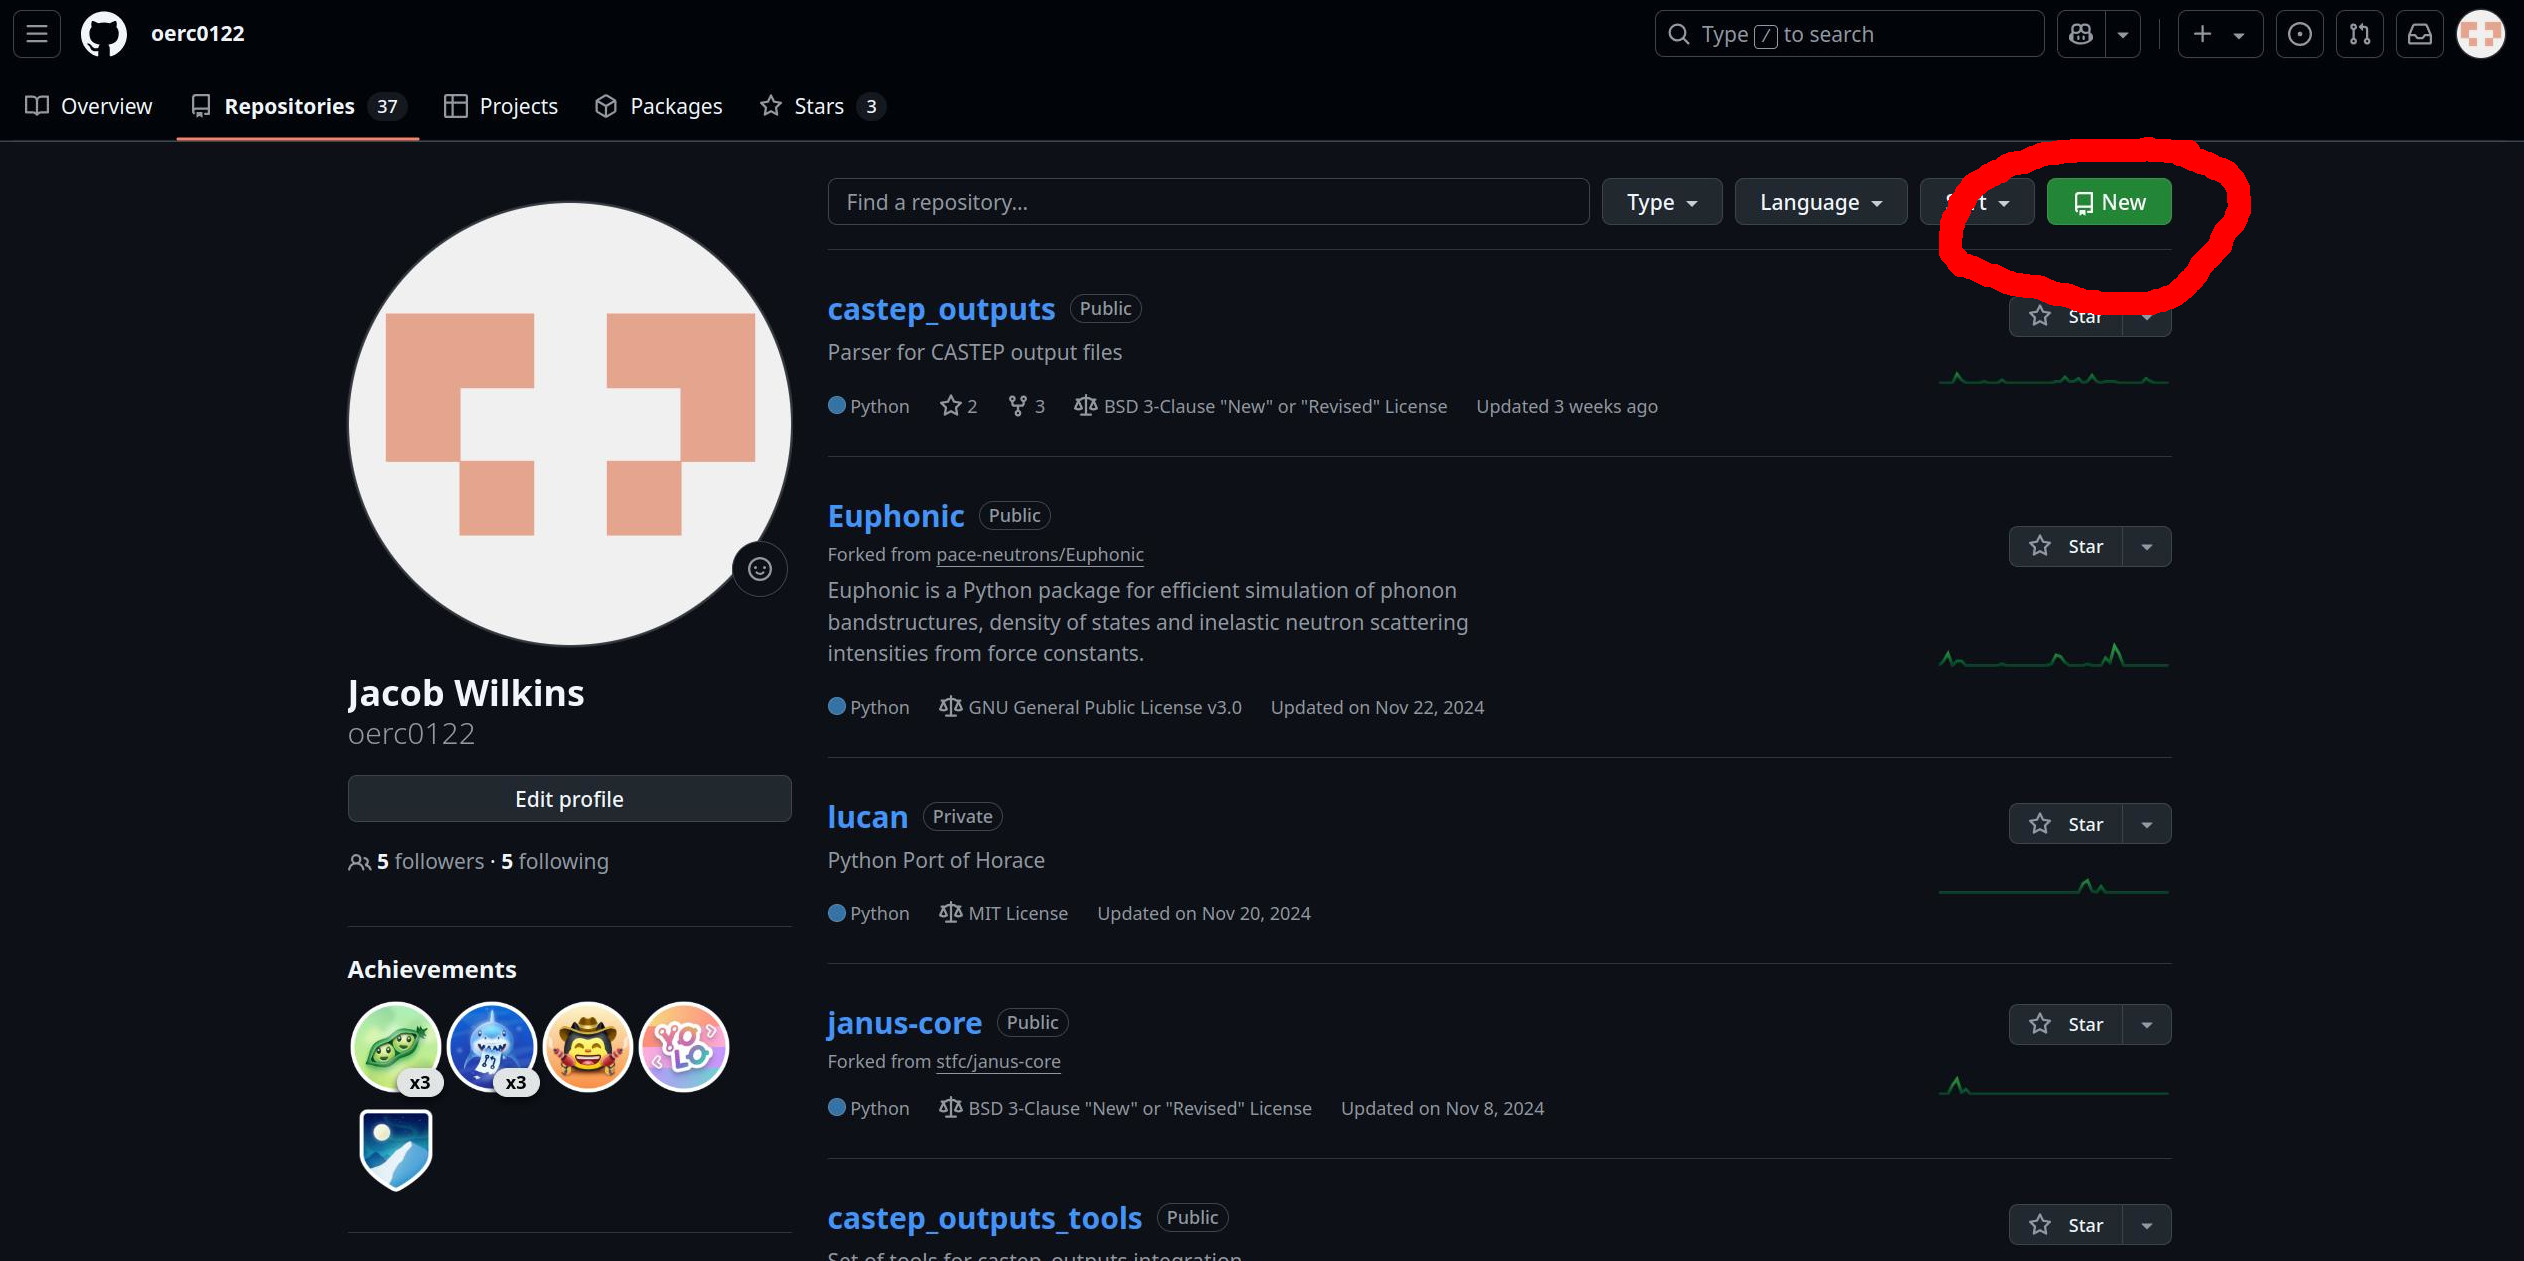
\includegraphics[width=0.9\textwidth]{new-repo.jpg}
        \end{center}
    }
    \only<2-5> {
        \vspace{-3em}
        \begin{center}
            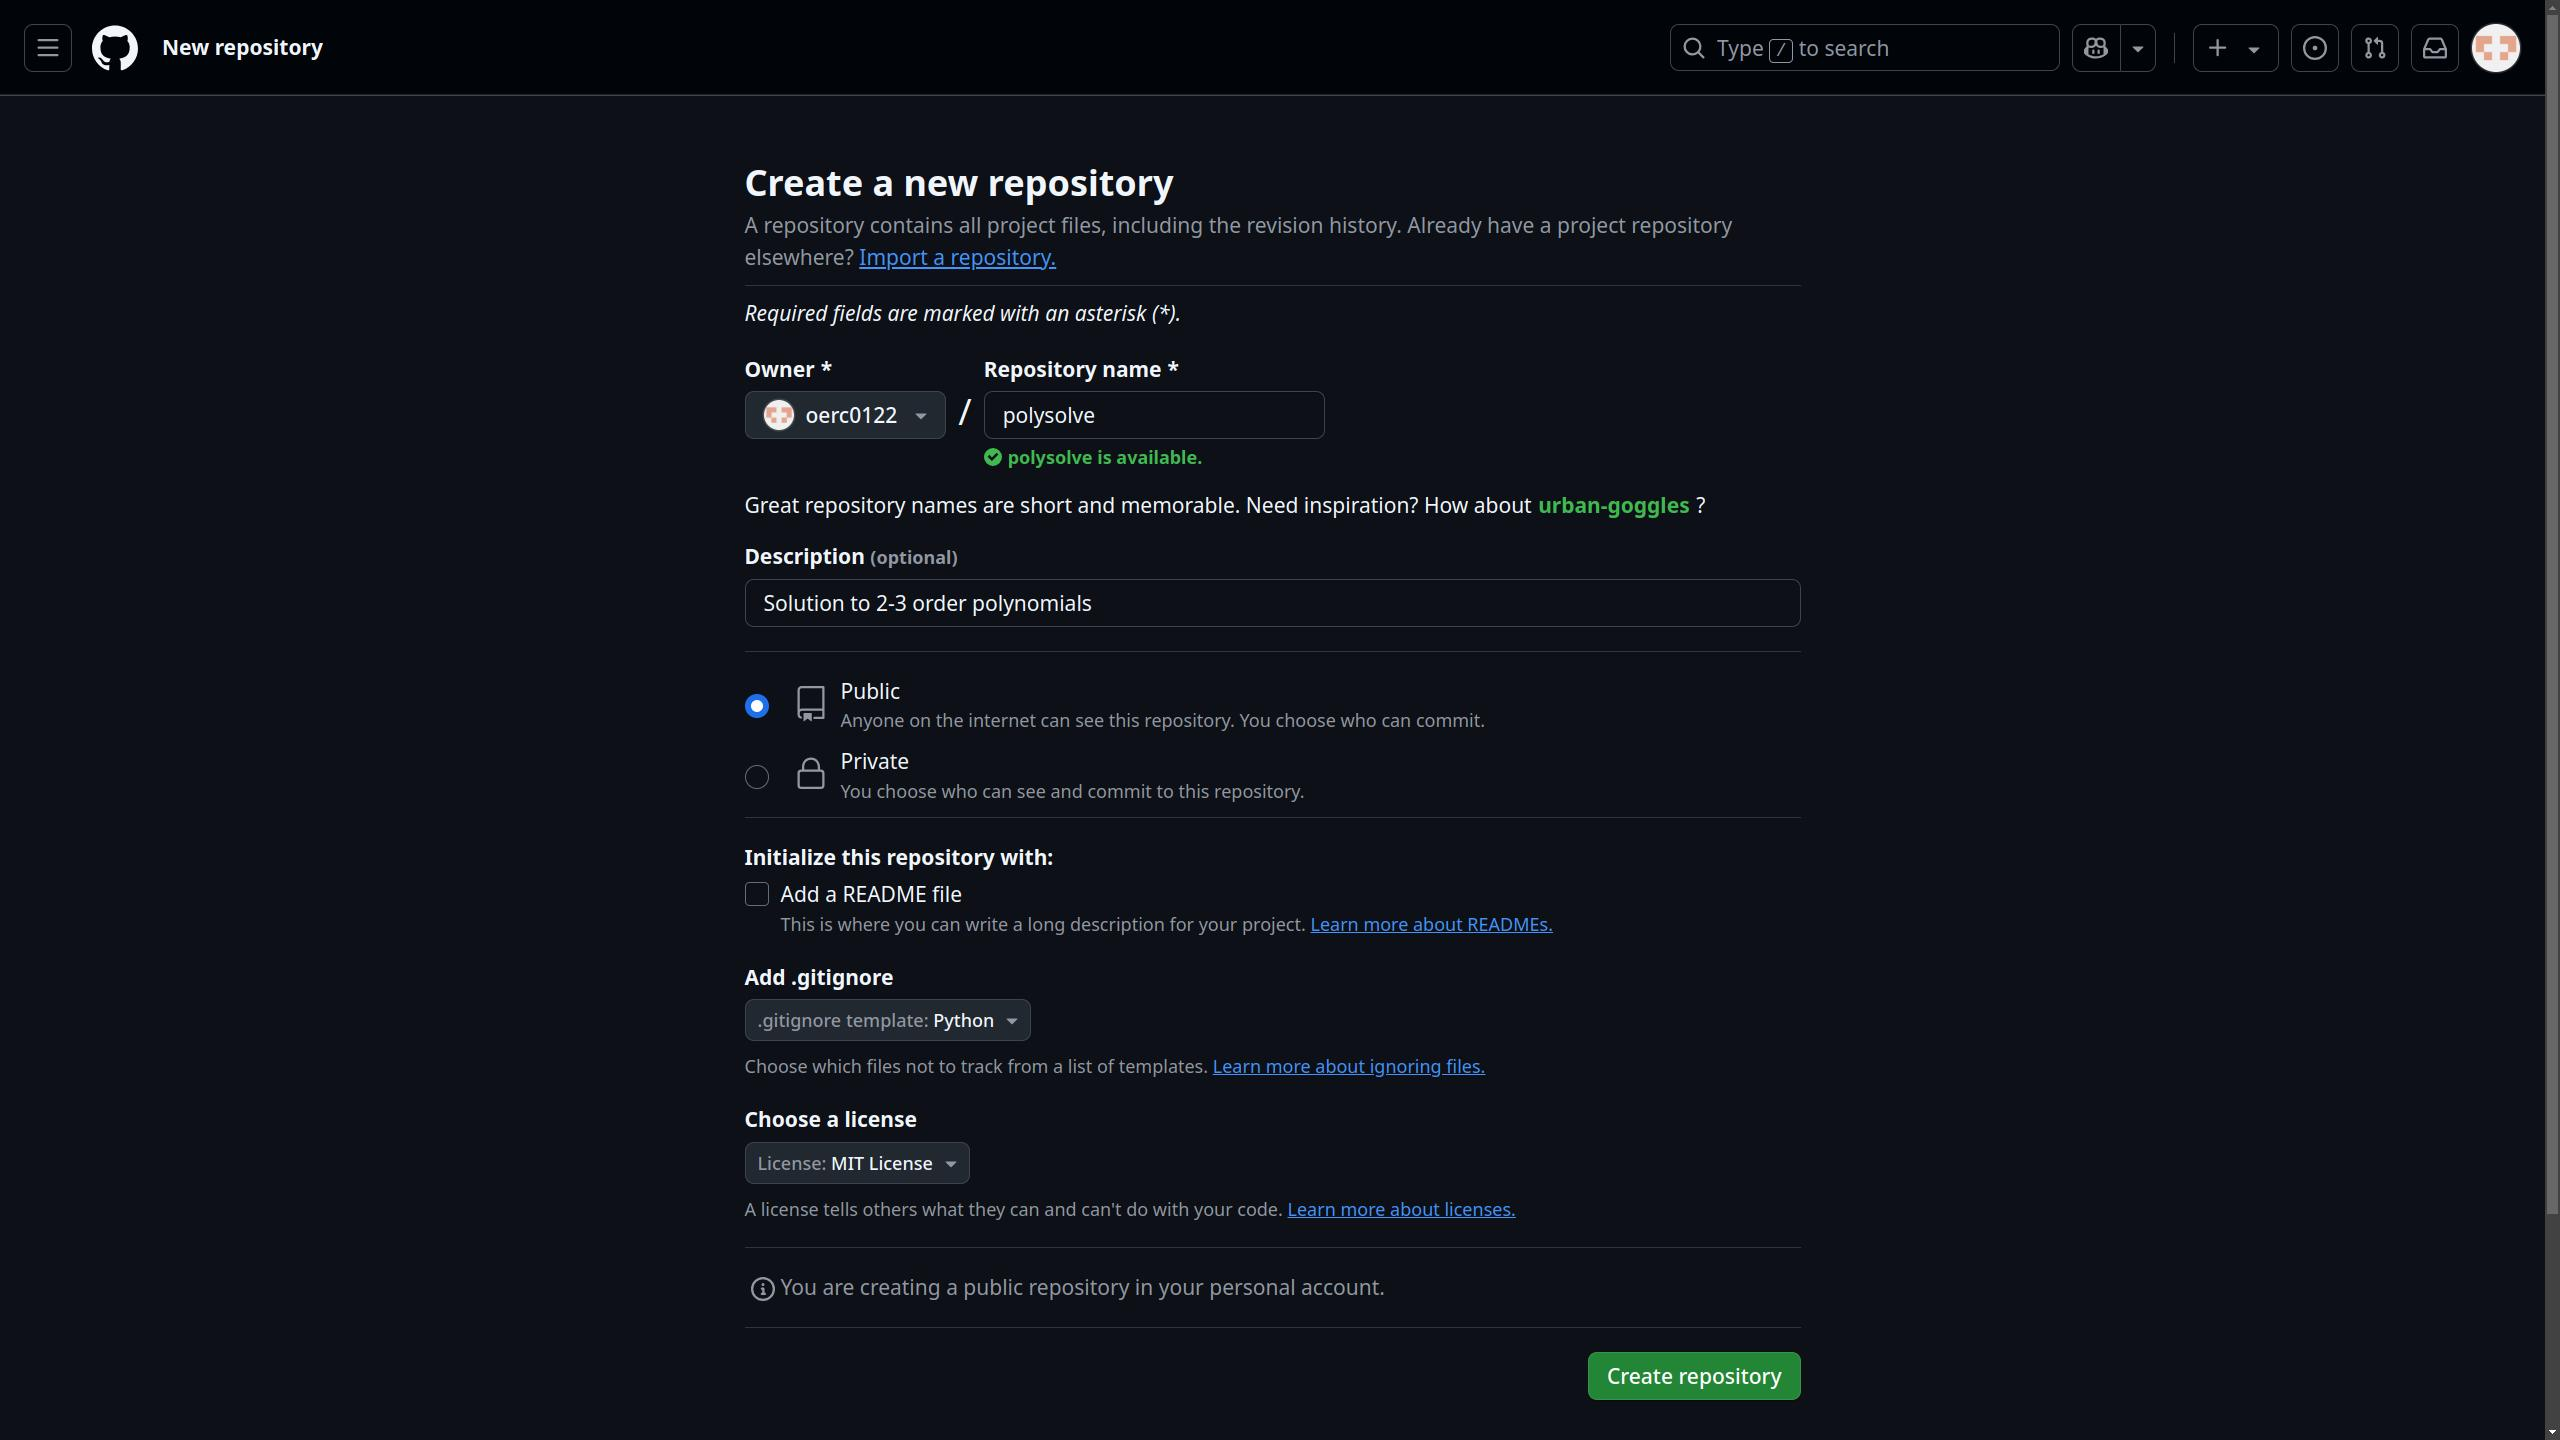
\includegraphics[width=0.9\textwidth]{creatingrepo.jpg}
        \end{center}
    }
\end{frame}

\begin{frame}{Using GitHub}
    \begin{itemize}[<+->]
        \item{}Double check on GitHub and your files should be on it.
    \end{itemize}
\end{frame}

\section{Package}

\subsection{init.py}

\begin{frame}{From script to project}
    \begin{itemize}[<+->]
        \item{}To start a project, we need to define what the project is.
        \item{}The first step is to change the structure to that of a project.
        \item{}Make a new folder ``\foldt{polysolve}'' and \cmd{git mv}  ``\filet{polysolve.py}'' into it.  
    \end{itemize}

    \begin{block}<+>{Layout}
    This form of putting code in \foldt{<project>/...} is called flat-layout.
    
    You can also put code in \foldt{src/<project>/...} this is called source-layout.
    \end{block}
\end{frame}

\begin{frame}{Making a package}
    \begin{itemize}[<+->]
        \item{}Now we add a new file called \initf{} in \foldt{polysolve}.
        \item{}The \initf{} is a magic file.
        \item{}In Python it makes a folder accessible for \kw{import}.
    \end{itemize}

    \begin{block}<+>{Try it out!}
        \lstinputlisting{import.py}
        
        \textbf{NOTE:} This is only accessible from our project folder, not the system, it's not installed yet.
    \end{block}
\end{frame}

\begin{frame}{Making a package}
    \begin{itemize}[<+->]
        \item{}All files in the folder with the \initf{} are accessible.
        \item{}Subfolders can be nested, each one needs an \initf{}.
        \item{}Code in an \initf{} is run \textbf{when the module is imported}.
        \item{}This can be used for setup or our package's metadata.
    \end{itemize}

    \begin{alertblock}<+>{Add some code to \_\_init\_\_.py}
    \lstinputlisting{__init__.py}
    \end{alertblock}
\end{frame}

\subsection{pyproject.toml}

\begin{frame}{Making a project}
    \begin{itemize}[<+->]
        \item{}Now that we have a package it's time to make this a project.
        \item{}We need a \filet{pyproject.toml}.
        \item{}\filet{pyproject.toml} defines the metadata our project\footnote{For more info on Python packaging take a look on the PyPA at: \\
    \scriptsize{\url{https://packaging.python.org/en/latest/tutorials/packaging-projects/}}}.
        \item{}When you \cmd{pip install} this reads the \filet{pyproject.toml}.
    \end{itemize}

    \begin{block}<2->{TOML History}
        TOML (Tom's Own Markup Language) is a standardised format designed to replace the non-standardised \filet{.ini} format configurations.
    \end{block}

    \begin{block}<+->{Ancient (modern) History}
        Older projects used to use something called \filet{setup.py}, this is being deprecated except where your project needs e.g. Cython or compiled C++, and even then...
    \end{block}

\end{frame}


\begin{frame}{The pyproject.toml}
    \lstinputlisting[basicstyle=\tiny]{pyproject.toml}

    Let's look at these individually.
    \begin{block}{Note}
        Keywords are arranged into ``block''s and are order independent within blocks. Blocks are order independent too.
    \end{block}
\end{frame}

\begin{frame}{build-system}
    \lstinputlisting[linerange={1-3}]{pyproject.toml}
    \begin{itemize}[<+->]
        \item{}These are the Python tools \cmd{pip} will use to build your project.
        \item{}You may choose something else (info on PyPA\footnote{\tiny{\url{https://packaging.python.org/en/latest/tutorials/packaging-projects/}}}), but we'll just stick with \cmd{setuptools}.
    \end{itemize}
\end{frame}

\begin{frame}{project}
    \lstinputlisting[linerange={5-15}]{pyproject.toml}
    \begin{itemize}
        \item{}These define the properties which describe your project:
        \only<+>{\item{}\kw{name} -- The project's installed name.}
        \only<+>{\item{}\kw{authors} -- The project's authors.*}
        \only<+>{\item{}\kw{requires-python} -- The minimum version of python needed to run the project.}
        \only<+>{\item{}\kw{readme} -- The readme file/content.*}
        \only<+>{\item{}\kw{description} -- A brief summary of the project.*}
        \only<+>{\item{}\kw{license} -- Project license.*}
        \only<+>{\item{}\kw{keywords} -- Searchable keywords describing project.*}
        \only<+>{\item{}\kw{classifiers} -- Set of keyword identifiers (see PyPA).*}
        \only<+>{\vspace{-1.2em}\item{}\kw{dependencies} -- List of project dependencies.}
    \end{itemize}
    \begin{block}{Note}
        * PyPI/repository only.
    \end{block}
\end{frame}

\begin{frame}{Webpages}
    \lstinputlisting[linerange={18-20}]{pyproject.toml}
    \begin{itemize}[<+->]
        \item{}PyPI will add these links in a sidebar if you upload your project.
    \end{itemize}
\end{frame}

\begin{frame}{Dynamic}
    \lstinputlisting[linerange={5,16,21-23}]{pyproject.toml}
    \begin{itemize}[<+->]
        \item{}You may have spotted \kw{dynamic} at the end of the \kw{[project]} block.
        \item{}\kw{dynamic} is a special keyword which tells \cmd{pip} the variable will come from somewhere else.
        \item{}We define our \kw{version} as coming from our package.
    \end{itemize}

    \begin{block}<+>{Extra dynamicism}
        We can define several other properties as \kw{dynamic} see PyPA for more info.
    \end{block}
\end{frame}

\begin{frame}{Connect the dots}
    \begin{itemize}[<+->]
        \item{}Copy \filet{pyproject.toml} to your project root directory.
        \item{}We can fill in the gaps in our \filet{pyproject.toml}
        \item{}\textbf{Note:} you need to have \kw{dependencies = ["numpy"]}
        \item{}Then we can see some magic happen.
        \item{}\cmd{pip} checks we have all the requirements, installs the dependencies, then our project.
        \item{}\textbf{NOTE:} It's now installed system-wide.
    \end{itemize}
    \only<2-4>{
        \begin{block}{Try it out!}
            \cmd{pip install .}
            
            \cmd{python}
            
            \cmd{>>> from polysolve import polysolve}
            
            \cmd{>>> polysolve.quadratic(3, 1, 2)}
        \end{block}
    }
    \begin{block}<5>{Developing}
        While developing you will want:
        
        \cmd{pip install -e .}
        
        which will link to the package so as you edit it the system version updates.
    \end{block}
\end{frame}

\begin{frame}{Get it gitted}
    \begin{itemize}[<+->]
        \item{}Now add the \filet{pyproject.toml} to \cmd{git}.
        \item{}Push it up to GitHub.
    \end{itemize}
    \only<3->{
        \begin{block}{More magic!}
            {\scriptsize \cmd{pip install git+https://github.com/<owner_name>/polysolve.git}
            
            \textbf{NOTE:} PyPI is ``easier'', but requires accounts. This is convenient for small stuff.}
        \end{block}
    }
\end{frame}

\begin{frame}{Great, we have a project}
    \begin{itemize}[<+->]
        \item{}Now what?
        \item{}The next step is to make it usable.
        \item{}That means usable by other people.
    \end{itemize}
\end{frame}

\section{Documentation}

\begin{frame}{Documentation, documentation, documentation.}
    \begin{itemize}[<+->]
        \item{}We're going to begin by looking at documentation.
        \item{}Documentation tends to fall by the wayside.
        \item{}\textbf{However}, it's the most important thing in released software.
    \end{itemize}
\end{frame}

\begin{frame}{Documentation, documentation, documentation.}
    \begin{itemize}[<+->]
        \item{}Let's start with something simple.
        \item{}Our \filet{README.md} basically says the project name.
        \item{}We know how to install it now, so let's add that.
        \item{}Push it up to GitHub and see the glory of your hard work.
    \end{itemize}

    \only<3->{
        \begin{block}{More magic!}
            {\scriptsize \cmd{pip install git+https://github.com/<owner_name>/polysolve.git}}
        \end{block}
    }   
\end{frame}

\subsection{Type-hints}

\begin{frame}{IDE Ahoy}
    \begin{itemize}[<+->]
        \item{}Anybody here used VSCode or another IDE\footnote{Interactive Development Environment}?
        \item{}When you start typing a function, it tells you what argument comes next.
        \item{}It also tells you the \kw{type} it should be (\kw{int}, \kw{float}, etc.).
    \end{itemize}
\end{frame}

\begin{frame}[fragile]{IDE Ahoy}
    \begin{itemize}[<+->]
        \item{}The IDE isn't doing any \textbf{magic} to find out, we tell it!
        \item{}How do we tell it?
        \item{}We use ``type-hints'' or ``annotations''.
    \end{itemize}

    \begin{onlyenv}<3>
        \begin{lstlisting}[basicstyle=\scriptsize]
def quadratic(
        a: float, 
        b: float, 
        c: float,
) -> tuple[float, float]:
    det = b**2 - (4*a*c)

    return ((-b + np.sqrt(det)) / (2*a),
            (-b - np.sqrt(det)) / (2*a))
        \end{lstlisting}
    \end{onlyenv}

    \begin{onlyenv}<4>
        \begin{lstlisting}[basicstyle=\scriptsize]
from __future__ import annotations
        
def quadratic(
        a: float, 
        b: float, 
        c: float,
) -> tuple[float, float]:
    det = b**2 - (4*a*c)

    return ((-b + np.sqrt(det)) / (2*a),
            (-b - np.sqrt(det)) / (2*a))
        \end{lstlisting}

        \begin{block}{Note}
            You may find on older Python versions for complex annotations you need to 
            \kw{import annotations}
        \end{block}
    \end{onlyenv}
\end{frame}

\begin{frame}[fragile]{Handy dandy}
    \begin{itemize}[<+->]
        \item{}These type-hints aren't just useful to users.
        \item{}They're useful to us as developers.
        \item{}We know when changing things what we're allowed to do.
    \end{itemize}

    \begin{lstlisting}[basicstyle=\scriptsize]
def quadratic(
        a: float, 
        b: float, 
        c: float,
) -> tuple[float, float]:
    det = b**2 - (4*a*c)

    return ((-b + np.sqrt(det)) / (2*a),
            (-b - np.sqrt(det)) / (2*a))
    \end{lstlisting}

\end{frame}

\subsection{Docstrings}

\begin{frame}{What are we doing again?}
    \begin{itemize}[<+->]
        \item{}So we know what we're feeding the black box.
        \item{}Wouldn't it be nice if the box told us what it did (or is trying to do)?
        \item{}Don't go rushing off to write in the filet{README.md} again!
    \end{itemize}
\end{frame}

\begin{frame}{What are we doing again?}
    \begin{itemize}[<+->]
        \item{}Python allows us to annotate further!
        \item{}Introducing the docstring!
        \item{}This is the minimal docstring.
        \item{}We can add more!\footnote{See \filet{quadexm.py}}
    \end{itemize}

    \begin{onlyenv}<2->
        \lstinputlisting[basicstyle=\scriptsize,linerange={3-5,51}]{quadexm.py}
    \end{onlyenv}
\end{frame}

\begin{frame}{What are we doing again?}
    \begin{itemize}[<+->]
        \item{}We can add more!\footnote[5]{See \filet{quadexm.py}}
    \end{itemize}

    % Basic
    \begin{onlyenv}<1>
        \lstinputlisting[basicstyle=\scriptsize,linerange={3-5,51}]{quadexm.py}
    \end{onlyenv}
    % Extended
    \begin{onlyenv}<+>
        \lstinputlisting[basicstyle=\scriptsize,linerange={3-7,51}]{quadexm.py}
    \end{onlyenv}
    % Params
    \begin{onlyenv}<+>
        \lstinputlisting[basicstyle=\scriptsize,linerange={3-17,51}]{quadexm.py}
    \end{onlyenv}
    % Returns
    \begin{onlyenv}<+>
        \lstinputlisting[basicstyle=\scriptsize,linerange={3-21,51}]{quadexm.py}
    \end{onlyenv}
    % Examples
    \begin{onlyenv}<+>
        \lstinputlisting[basicstyle=\scriptsize,linerange={36-41}]{quadexm.py}
    \end{onlyenv}
    % Raises
    \begin{onlyenv}<+>
        \lstinputlisting[basicstyle=\scriptsize,linerange={22-26}]{quadexm.py}
    \end{onlyenv}
    % Notes
    \begin{onlyenv}<+>
        \lstinputlisting[basicstyle=\scriptsize,linerange={27-34}]{quadexm.py}
    \end{onlyenv}
    % See Also
    \begin{onlyenv}<+>
        \lstinputlisting[basicstyle=\scriptsize,linerange={43-46}]{quadexm.py}
    \end{onlyenv}
    % References
    \begin{onlyenv}<+>
        \lstinputlisting[basicstyle=\scriptsize,linerange={47-50}]{quadexm.py}
    \end{onlyenv}
\end{frame}

\begin{frame}[fragile]{Substance over style}
    \begin{itemize}[<+->]
        \item{}\textbf{Note:} what I've been showing you is \textbf{one} style of docs.
        \item{}This style is called \kw{numpydoc} style after the \cmd{numpy} library.
    \end{itemize}
\end{frame}

\begin{frame}[fragile]{Substance over style}
    The main styles are: 
    \kw{numpydoc} \\
    {\footnotesize \url{numpydoc.readthedocs.io/en/latest/format.html}}

    \lstinputlisting[basicstyle=\tiny,linerange={3-21,51}]{quadexm.py}

\end{frame}
    
\begin{frame}[fragile]{Substance over style}
    The main styles are: 
    \kw{google} \\ 
    {\footnotesize \url{google.github.io/styleguide/pyguide.html}}

    \begin{lstlisting}[basicstyle=\scriptsize]
def quadratic(a: float, b: float, c: float) -> tuple[float, float]:
    """Solves the roots of a quadratic equation.

    Uses the quadratic formula. Result must be real.

    Parameters:
        a: :math:`x^2` coefficient.
        b: :math:`x` coefficient.
        c: Constant value.
    
    Returns:
        Positive and negative roots of quadratic.
    """
    \end{lstlisting}

\end{frame}

\begin{frame}[fragile]{Substance over style}
    The main styles are: 
    \kw{sphinx} \\ 
    {\footnotesize \url{sphinx-rtd-tutorial.readthedocs.io/en/latest/docstrings.html}}

    \begin{lstlisting}[basicstyle=\scriptsize]
def quadratic(a: float, b: float, c: float) -> tuple[float, float]:
    """Solves the roots of a quadratic equation.

     Uses the quadratic formula. Result must be real.
     
    :param a: :math:`x^2` coefficient.
    :param b: :math:`x` coefficient.
    :param c: Constant value.
    
    :return: Positive and negative roots of quadratic.
    """
    \end{lstlisting}

\end{frame}

\subsection{Doctests}

\begin{frame}{More magic}
    \begin{itemize}[<+->]
        \item{}Ok, we've got docstrings. Now time for a callback:
        \item{}Remember this?\footnote[5]{See \filet{quadexm.py}}
        \item{}What happens if this goes out of date or doesn't work?
    \end{itemize}

    \begin{onlyenv}<2->
        \lstinputlisting[basicstyle=\scriptsize,linerange={36-41}]{quadexm.py}
    \end{onlyenv}
\end{frame}

\begin{frame}[fragile]{More magic}
    \begin{itemize}[<+->]
        \item{}Thankfully, Python provides a way to use these as tests!
        \item{}{\scriptsize (Already into tests and we're not out of the docs section yet! Sneak peek!)}
        \item{}\url{https://docs.python.org/3/library/doctest.html}
    \end{itemize}

    \lstinputlisting[basicstyle=\scriptsize,linerange={36-41}]{quadexm.py}

    \begin{onlyenv}<+>
        \begin{block}{Try it out!}
            \begin{lstlisting}
python -m doctest polysolve.py
            \end{lstlisting}
        \end{block}
    \end{onlyenv}
        
    \begin{onlyenv}<+>
        \begin{block}{Try it out!}
            \begin{lstlisting}
if __name__ == "__main__":
    import doctest
    doctest.testmod()

python polysolve.py
            \end{lstlisting}
        \end{block}
    \end{onlyenv}
\end{frame}

\begin{frame}[fragile]{More magic}
    \begin{itemize}[<+->]
        \item{}Doctests are designed to imitate Python REPL.
        \item{}Designed for copying and pasting from REPL.
        \item{}Lines starting with ``\kw{>>>}'' are run.
        \item{}Lines can be continued/indented with ``\kw{...}''.
        \item{}Lines with neither are checked against the result.
        \item{}Need to import libraries if they're needed.
    \end{itemize}

    \begin{onlyenv}<1-5>
        \begin{block}{Example}
            \begin{lstlisting}
>>> my_var = ["hello", "goodbye"]
>>> my_var
['hello', 'goodbye']
>>> for i in range(3):
...     print(i)
0
1
2
            \end{lstlisting}
        \end{block}
    \end{onlyenv}

    \begin{onlyenv}<6>
        \begin{block}{Example}
            \begin{lstlisting}
>>> import numpy as np
>>> np.array([1, 2, 3])
array([1, 2, 3])
            \end{lstlisting}
        \end{block}
    \end{onlyenv}

    \begin{onlyenv}<+>
        \begin{block}{Fun (useful) (magic?) fact}
            Doctest doesn't care about what strings its reading and will read and run 
            any \cmd{>>>} style stuff even in documentation or text files!
            \\\ \\
            \cmd{python} \kw{-m} \kw{doctest} \filet{my_text.txt}
        \end{block}
    \end{onlyenv}
    
\end{frame}

\subsection{Sphinx}

\begin{frame}[fragile]{Finally getting to docs}
    \begin{itemize}[<+->]
        \item{}Now after so long, it's time to finally write some docs!
        \item{}{\small (or let the computer write some for us...)}
    \end{itemize}
    
    \begin{block}<+>{Getting started! (Linux)}
        \begin{lstlisting}[language=sh]
pip install sphinx sphinx_rtd_theme
mkdir docs; cd docs
sphinx-quickstart
make html
chromium build/html/index.html
        \end{lstlisting}
    \end{block}
\end{frame}

\begin{frame}{Keys to the docs}
    \begin{itemize}[<+->]
        \item{Key files in the new docs are:}
        \begin{itemize}
            \item{}\filet{conf.py} -- Configuration for docs.
            \item{}\filet{index.rst} -- Main starting file for docs.
        \end{itemize}
        \item{}Let's take a look at these.
    \end{itemize}
\end{frame}

\begin{frame}{conf.py}
    \begin{itemize}[<+->]
        \item{}\filet{conf.py} is an auto-generated Python file with instructions for building the docs.
        \item{}It is a full Python file you can run code in, e.g. we can pull out information from our package.
        \item{}For example, we can use our defined metadata.
        \item{}\cmd{sphinx} is a fully extensible package. We'll be using some of these later.
        \item{}\kw{exclude_patterns} allows us to exclude source files from our sphinx build.
        \item{}We can change the docs theme to render them differently.
        \item{}Since we installed \kw{sphinx_rtd_theme} we can try that.
    \end{itemize}

    \only<1-2>{\lstinputlisting[basicstyle=\tiny,linerange={1-5}]{conf.py}}
    \only<3>{\lstinputlisting[basicstyle=\tiny,linerange={6-14}]{conf.py}}
    \only<4-5>{\lstinputlisting[basicstyle=\tiny,linerange={16-22}]{conf.py}}
    \only<6-7>{\lstinputlisting[basicstyle=\tiny,linerange={24-28}]{conf.py}}
\end{frame}

\begin{frame}{index.rst}
    \begin{itemize}[<+->]
        \item{}\cmd{sphinx} docs are written in REStructured Text (ReST/rst)\footnote{{\scriptsize \url{www.sphinx-doc.org/en/master/usage/restructuredtext/index.html}}}.
        \item{}Text ``marked-up'' with formatting (like \LaTeX{} or HTML).
    \end{itemize}

    \lstinputlisting[basicstyle=\tiny,linerange={-16}]{index.rst}
\end{frame}

\begin{frame}[fragile]{Writing our docs}
    \begin{itemize}
        \item<1->{}Now we need some files to actually to actually fill with docs!
        \item<2->{}Create a file called \filet{usage.rst}.
        \item<3->{}Write some documentation.
        \item<4->{}Add it to our ``table of contents tree'' (\kw{toctree}).
        \item<6->{}Build our docs!
    \end{itemize}

    \begin{onlyenv}<3>
        \begin{lstlisting}
Usage
=====

Here's how to use polysolve!
        \end{lstlisting}
    \end{onlyenv}
    
    \only<4>{\lstinputlisting[linerange={14-16}]{index.rst}}
    \only<5>{\lstinputlisting[linerange={14-18}]{index.rst}}
    \begin{onlyenv}<6>
        \begin{block}{Make it so!}
            \cmd{make html}
        \end{block}
    \end{onlyenv}
    
\end{frame}

\subsection{Sphinx Autodocs}

\begin{frame}{Docstring Magic}
    \begin{itemize}[<+->]
        \item{}So now we can write about every single function in our project.
        \begin{itemize}
            \item{}How many could there be?
            \item{}What do you mean not every project has 20 lines?
        \end{itemize}
        \item{}Remember our docstrings?
        \item{}Maybe there's a way to avoid writing everything twice.
    \end{itemize}
\end{frame}

\begin{frame}{Docstring magic}
    \begin{itemize}[<+->]
        \item{}What if we could extract all the docstrings we've already written?
        \item{}We're going to need to do a couple of things.
        \item{}Time to use some extensions.
        \item{}\kw{sphinx.ext.autodoc} extracts docstrings from functions.
        \item{}\kw{sphinx.ext.napoleon} converts our \cmd{numpydoc} to \cmd{sphinx}
        \item{}\kw{sphinx.ext.autosummary} adds a summary to each page.
    \end{itemize}

    \begin{onlyenv}<3->
        \texttt{extensions = [
            \only<4->{ \\"sphinx.ext.autodoc",\\}
            \only<5->{"sphinx.ext.napoleon",\\}
            \only<6->{"sphinx.ext.autosummary",\\}
        ]
            }
    \end{onlyenv}
\end{frame}

\begin{frame}{Docstring magic}
    \begin{itemize}[<+->]
        \item{}We need to create all the infrastructure to extract our info.
        \item{}Just kidding, there's a tool for that!
        \item{}Just add it to the \cmd{toctree} and we're set.
        \item{}{\scriptsize after we \cmd{make html}}
    \end{itemize}

    \only<2>{
        \begin{block}{It's magic!}
            \cmd{sphinx-apidoc -o docs/source/api polysolve}
        \end{block}
    }
    \only<3>{\lstinputlisting[linerange={14-19}]{index.rst}}
\end{frame}

\begin{frame}[fragile]{Type-hints}
    \begin{itemize}[<+->]
        \item{}But our typehints aren't with our params...
        \item{}If only there were some tool to extract those too.
        \item{}Alas, it's surely impossible...
    \end{itemize}

    \begin{onlyenv}<+>
        \begin{block}{Da-da-da-daaaa}
            \cmd{pip install sphinx-autodoc-typehints}
        \end{block}
    \end{onlyenv}

    \begin{onlyenv}<+>
        \begin{block}{Da-da-da-daaaa}
            \begin{lstlisting}
extensions = [...,
              "sphinx_autodoc_typehints",
              ]
            \end{lstlisting}
        \end{block}
    \end{onlyenv}

\end{frame}

\subsection{intersphinx}

\begin{frame}[fragile]{But what is a float really?}
    \begin{itemize}[<+->]
        \item{}But now I'm unhappy because when I click \kw{float} it doesn't take me to the documentation of \kw{float}.
        \item{}{\scriptsize Some people, honestly.}
        \item{}Introducing ``\cmd{intersphinx}''.
        \item{}Links your documentation against other \cmd{sphinx} documentation sites automatically.
    \end{itemize}

    \begin{onlyenv}<3->
        \begin{block}{Ta-da}
            \begin{lstlisting}[basicstyle=\tiny]
extensions = [...,
              "sphinx.ext.intersphinx",
              ]
              ...
intersphinx_mapping = {'python': ('https://docs.python.org/3/', None),
                       'numpy': ('https://docs.scipy.org/doc/numpy/', None),
                       ...}
            \end{lstlisting}
        \end{block}
    \end{onlyenv}    
\end{frame}

\begin{frame}[fragile]{Adding it to the project}
    \begin{itemize}[<+->]
        \item{}Now that we know what we need, we can add these to our \filet{pyproject.toml}.
        \item{}Not everyone needs to install them, so let's add them as an optional dependency.
    \end{itemize}

    \begin{onlyenv}<+>
        \begin{block}{Adding it in}
            \begin{lstlisting}[basicstyle=\scriptsize]
[project.optional-dependencies]
docs = ["sphinx",
        "sphinx_rtd_theme", 
        "sphinx_autodoc_typehints"]
            \end{lstlisting}
        \end{block}
    \end{onlyenv}

    \begin{onlyenv}<+>
        \begin{block}{Adding it in}
            To install:

            \cmd{pip install -e ".[docs]"}
        \end{block}
    \end{onlyenv}    
\end{frame}


\begin{frame}{Done with docs}
    \begin{itemize}[<+->]
        \item{}More extensions and tools are available for building docs.
        \item{}In particular things like:
        \begin{itemize}
            \item{}Integrated Jupyter tutorials (\cmd{nbsphinx}).
            \item{}Testing within documentation (\cmd{sphinx.ext.doctest}).
            \item{}and many more...
        \end{itemize}
    \end{itemize}
\end{frame}

\section{Tests}

\begin{frame}{Done with docs}
    \begin{itemize}[<+->]
        \item{}Now we have some documentation to back up our code.
        \item{}Now we're ready to check it works.
        \item{}We already have \kw{doctest}s, which are good, but incomplete.
    \end{itemize}
\end{frame}

\begin{frame}{Types of tests}
    \begin{itemize}[<+->]
        \item{}We generally break testing down into 3--4 main types:
        \begin{itemize}
            \item{}Unit tests -- Tests of each function.
            \item{}System tests / End-to-end tests -- Small tests of the whole programs.
            \item{}Benchmark tests -- Tests real world cases.
            \item{}Integration tests -- Tests interfaces between program components.
        \end{itemize}
        \item{}We split these into three types:
        \begin{itemize}
            \item{}Science tests -- Check the validity against a known result.
            \item{}Regression tests -- Check values haven't changed.
            \item{}Fail-state tests -- Intentionally check failure states.
        \end{itemize}
    \end{itemize}
\end{frame}

\begin{frame}{Testing}
    \begin{itemize}[<+->]
        \item{}Our \kw{doctest}s go some of the way towards unit-tests.
        \item{}But they aren't the be all and end all.
        \item{}Let's see how to do proper tests.
    \end{itemize}
\end{frame}

\begin{frame}[fragile]{Testing}
    \begin{itemize}[<+->]
        \item{}First let's install the \kw{pytest}\footnote{\textbf{NOTE:} Python ships with the \kw{unittest} library, but rather than teaching two methods and confusing things, I'm sticking with one.} library.
        \item{}Let's create a \foldt{tests} folder.
        \item{}In that folder, let's create a \filet{test_quadratic.py}.
        \item{}What type of test is this?
        \item{}Run it!
        \item{}But what about our doctests?
    \end{itemize}

    \only<1>{
    \begin{block}{Let's get started!}
        \cmd{pip install pytest}
    \end{block}    
    }
    
    \begin{onlyenv}<3-4>
        \begin{lstlisting}[basicstyle=\tiny]
import pytest
import numpy as np
from polysolve.polysolve import quadratic

def test_quadratic():
    """Tests that quadratic finds the root for a known problem."""
    params = [3., 0., -1.]
    roots = quadratic(*params)
    assert all(np.isclose(np.polyval(params, root), 0.) for root in roots)
        \end{lstlisting}
    \end{onlyenv}

    \only<5>{
    \begin{block}{Try it out!}
        \cmd{pytest}
    \end{block}
    }

    \only<6>{
    \begin{block}{Try it out!}
        \cmd{pytest --doctest-modules}
    \end{block}
    }
\end{frame}

\begin{frame}{Testing}
    \begin{itemize}[<+->]
        \item{}\kw{pytest} picks up files called \filet{test_*}
        \item{}Runs all functions starting with \kw{test_}.
        \item{}{\scriptsize (and as mentioned with the \cmd{--doctest-modules} flag, runs those too)}
        \item{}Collates them all and runs them together.
    \end{itemize}
\end{frame}

\begin{frame}{Multiple-Testing}
    \begin{itemize}[<+->]
        \item{}So we have our first test, but solving $3x^2 - 1$ shouldn't be all we try.
        \item{}Try to think of all the common cases...
        \begin{enumerate}
            \item{}What other common cases might we try?
            \item{}What happens if $a = 0$?
            \item{}What happens if $b^2 - 4ac < 0$?
            \item{}What happens if I pass \kw{int}s?
            \item[$\vdots$]{}...
        \end{enumerate}
    \end{itemize}
\end{frame}

\begin{frame}[fragile]{Multiple-Testing}
    \begin{itemize}[<+->]
        \item{}Focussing on question 1...
        \item{}We want to run say: $x^2$, $x^2 + 14x + 49$, $3x^2 + 2x + 1$, ...
        \item{}Do we need to create a function for each one? \only<4->{No.}
    \end{itemize}

    \begin{onlyenv}<4>
        \begin{lstlisting}[basicstyle=\scriptsize]
@pytest.mark.parametrize('params, expected',
                         [([1., 0., 0.], [0., 0.]),
                          ([1., 14., 49.], [7., 7.]),
                          ([3., 2., 1.], [1/3, -1.])])
def test_quadratic(params, expected):
    """Test quadratic meets expectations."""
    assert np.isclose(quadratic(*params), expected)
        \end{lstlisting}
    \end{onlyenv}

    \begin{onlyenv}<5>
        \begin{lstlisting}[basicstyle=\scriptsize]
@pytest.mark.parametrize('a', [1, 2, 3])
@pytest.mark.parametrize('b', [1, 2, 3])
def test_example(a, b):
    """Example function taking 2 arguments."""
    assert np.product([a, b]) == a*b
        \end{lstlisting}
    
        \begin{block}{Note}
            Stacked \cmd{pytest.mark.parametrize}s give Cartesian product.
        \end{block}
    \end{onlyenv}
\end{frame}

\begin{frame}[fragile]{Testing failures}
    \begin{itemize}[<+->]
        \item{}Now we need to fail spectacularly.
        \item{}Usually, providing a wrong answer is worse than exploding\footnote{HCF - Halt and Catch Fire -- Genuine assembly instruction}.
        \item{}It's good to make sure our failures fail and are helpful.
        \item{}Does it fail?
    \end{itemize}

    \begin{onlyenv}<3->
        \begin{lstlisting}[basicstyle=\scriptsize]
def test_quadratic_fails():
    """Check bad quadratic raises error."""
    with pytest.raises(ValueError, 
                       match="negative discriminant"):
        # There are infinite roots on this flat line.
        quadratic(0., 0., 0.)
        \end{lstlisting}
    \end{onlyenv}
\end{frame}

\begin{frame}{Testing as design}
    \begin{itemize}[<+->]
        \item{}We should know what we want our code to do before we write it.
        \item{}One way of writing software is:
        \begin{itemize}
            \item{}Define tests which describe desired functionality.
            \item{}Develop until tests pass.
        \end{itemize}
        \item{}This can be useful for known problems.
        \item{}{\scriptsize Roughly describing something called Behaviour-Driven Development.}
    \end{itemize}
\end{frame}

\begin{frame}[fragile]{Testing}
    \begin{itemize}[<+->]
        \item{}Ok, I've written a test which doesn't work (yet).
        \item{}We can skip the test if we know it doesn't work (yet).
        \item{}It is bad practice to skip tests because they don't work.
        \item{}It is worse practice to remove tests because they don't work.
        \item{}Remove tests only if they don't fit the design.
    \end{itemize}

    \begin{onlyenv}<2->
        \begin{lstlisting}[basicstyle=\scriptsize]
@pytest.mark.skip(reason="Beyond maths as we know it.") 
def test_quintic():
    """Test quintic meets expectations."""
    assert np.isclose(quintic(1., 0., 0., 0., 0., 0., 0.), expected)
        \end{lstlisting}
    \end{onlyenv}
\end{frame}

\begin{frame}[fragile]{Testing}
    \begin{itemize}[<+->]
        \item{}Testing helps you:
        \begin{itemize}
            \item{}Prove the efficacy of your code.
            \item{}Develop functionality defined by requirements.
            \item{}Identify exactly when something went wrong.
            \item{}Avoid adding broken code.
        \end{itemize}
        \item{}\textbf{Hint:} Testing is good.
        \item{}Code without tests can be considered worthless.
        \item{}So let's add it to our \filet{pyproject.toml}
    \end{itemize}

    \begin{onlyenv}<8>
        \begin{block}{Adding it in}
            \begin{lstlisting}[basicstyle=\scriptsize]
[project.optional-dependencies]
docs = ["sphinx",
        "sphinx-rtd-theme", 
        "sphinx_autodoc_typehints"]
test = ["pytest"]
            \end{lstlisting}
        \end{block}
    \end{onlyenv}

\end{frame}

\begin{frame}{Testing}
    \begin{itemize}[<+->]
        \item{}As discussed a few other times \kw{pytest} is one of many testing frameworks. Others include:
        \item{}\kw{unittest} -- Basic test harness installed with \cmd{Python}.
        \item{}\kw{cucumber} -- Tests written in ``English'' rather than code.
        \item{}\kw{hypothesis} -- Tests with randomly generated values meeting requirements.
    \end{itemize}
\end{frame}

\section{CI/CD}

\begin{frame}{Automagic}
    \begin{itemize}[<+->]
        \item{}But running tests isn't fun.
        \item{}It'd be boring if we had to do it \textbf{every} time.
        \item{}If only there were a better way...
        \item{}CI/CD (continuous integration/continuous deployment)
        \item{}Fancy name which means automated testing \& building.
    \end{itemize}
\end{frame}

\begin{frame}{Automagic}
    \begin{itemize}[<+->]
        \item{}GitHub lets us run tests on their machines.
        \item{}{\small with some minor caveats}
        \item{}We just need to tell them what they need to do.
        \item{}We do this by adding a \filet{yaml} file in the right place.
        \item{}GitHub provides actions where we just need to fill in values.
    \end{itemize}

    \only<4>{
        \begin{block}{Adding it in!}
            \cmd{mkdir -P .github/workflows}
    
            \cmd{cp <pres>/test_florp.yml .github/workflows}
        \end{block}
    }
\end{frame}

\begin{frame}{Anatomy of the YAML}
    \begin{itemize}[<+->]
        \item{}Display name and script permissions.
        \item{}What will trigger the run.
        \begin{itemize}
            \item<.>{}When \kw{main} changes.
            \item<.>{}When a pull request is opened or changes.
        \end{itemize}            
        \item{}\vspace{-1.9\baselineskip}Main job description.
        \item{}Run on Ubuntu with each of the python versions
        \item{}Job stages using matrix defined previously.
        \begin{itemize}
            \item{}Download the repo using git
            \item<.->{}Install Python
            \item{}Install the project
            \item{}Run the tests.
        \end{itemize}
    \end{itemize}
    \only<1-3>{\vspace{-5\baselineskip}}
    \only<1>{\lstinputlisting[basicstyle=\tiny, linerange={4-7}]{test_florp.yml}}
    \only<2>{\lstinputlisting[basicstyle=\tiny, linerange={9-16}]{test_florp.yml}}
    \only<3>{\lstinputlisting[basicstyle=\tiny, linerange={18-39}]{test_florp.yml}}
    \only<4>{\lstinputlisting[basicstyle=\tiny, linerange={21-25}]{test_florp.yml}}
    \only<5>{\lstinputlisting[basicstyle=\tiny, linerange={27-39}]{test_florp.yml}}
    \only<6>{\lstinputlisting[basicstyle=\tiny, linerange={28-32}]{test_florp.yml}}
    \only<7>{\lstinputlisting[basicstyle=\tiny, linerange={34-36}]{test_florp.yml}}    
    \only<8>{\lstinputlisting[basicstyle=\tiny, linerange={38-40}]{test_florp.yml}}    
\end{frame}

\begin{frame}{Testing}
    \begin{itemize}[<+->]
        \item{}For more info see \\
        \url{https://docs.github.com/en/actions}
        \item{}There is a bit of magic, using other people's scripts.
        \begin{itemize}
            \item{}(The \cmd{actions/...@v3})
        \end{itemize}
        \item{}Besides that, it's just the commands you would run.
        \item{}GitHub offers Windows/Mac machines too!
    \end{itemize}
\end{frame}

\begin{frame}{Action Economy}
    \begin{itemize}[<+->]
        \item{}GitHub contains a number of pre-written scripts for doing common jobs.
        \item{}These can be useful starting points for writing more complex scripts yourself.
    \end{itemize}

    \only<1> {
        \begin{center}
            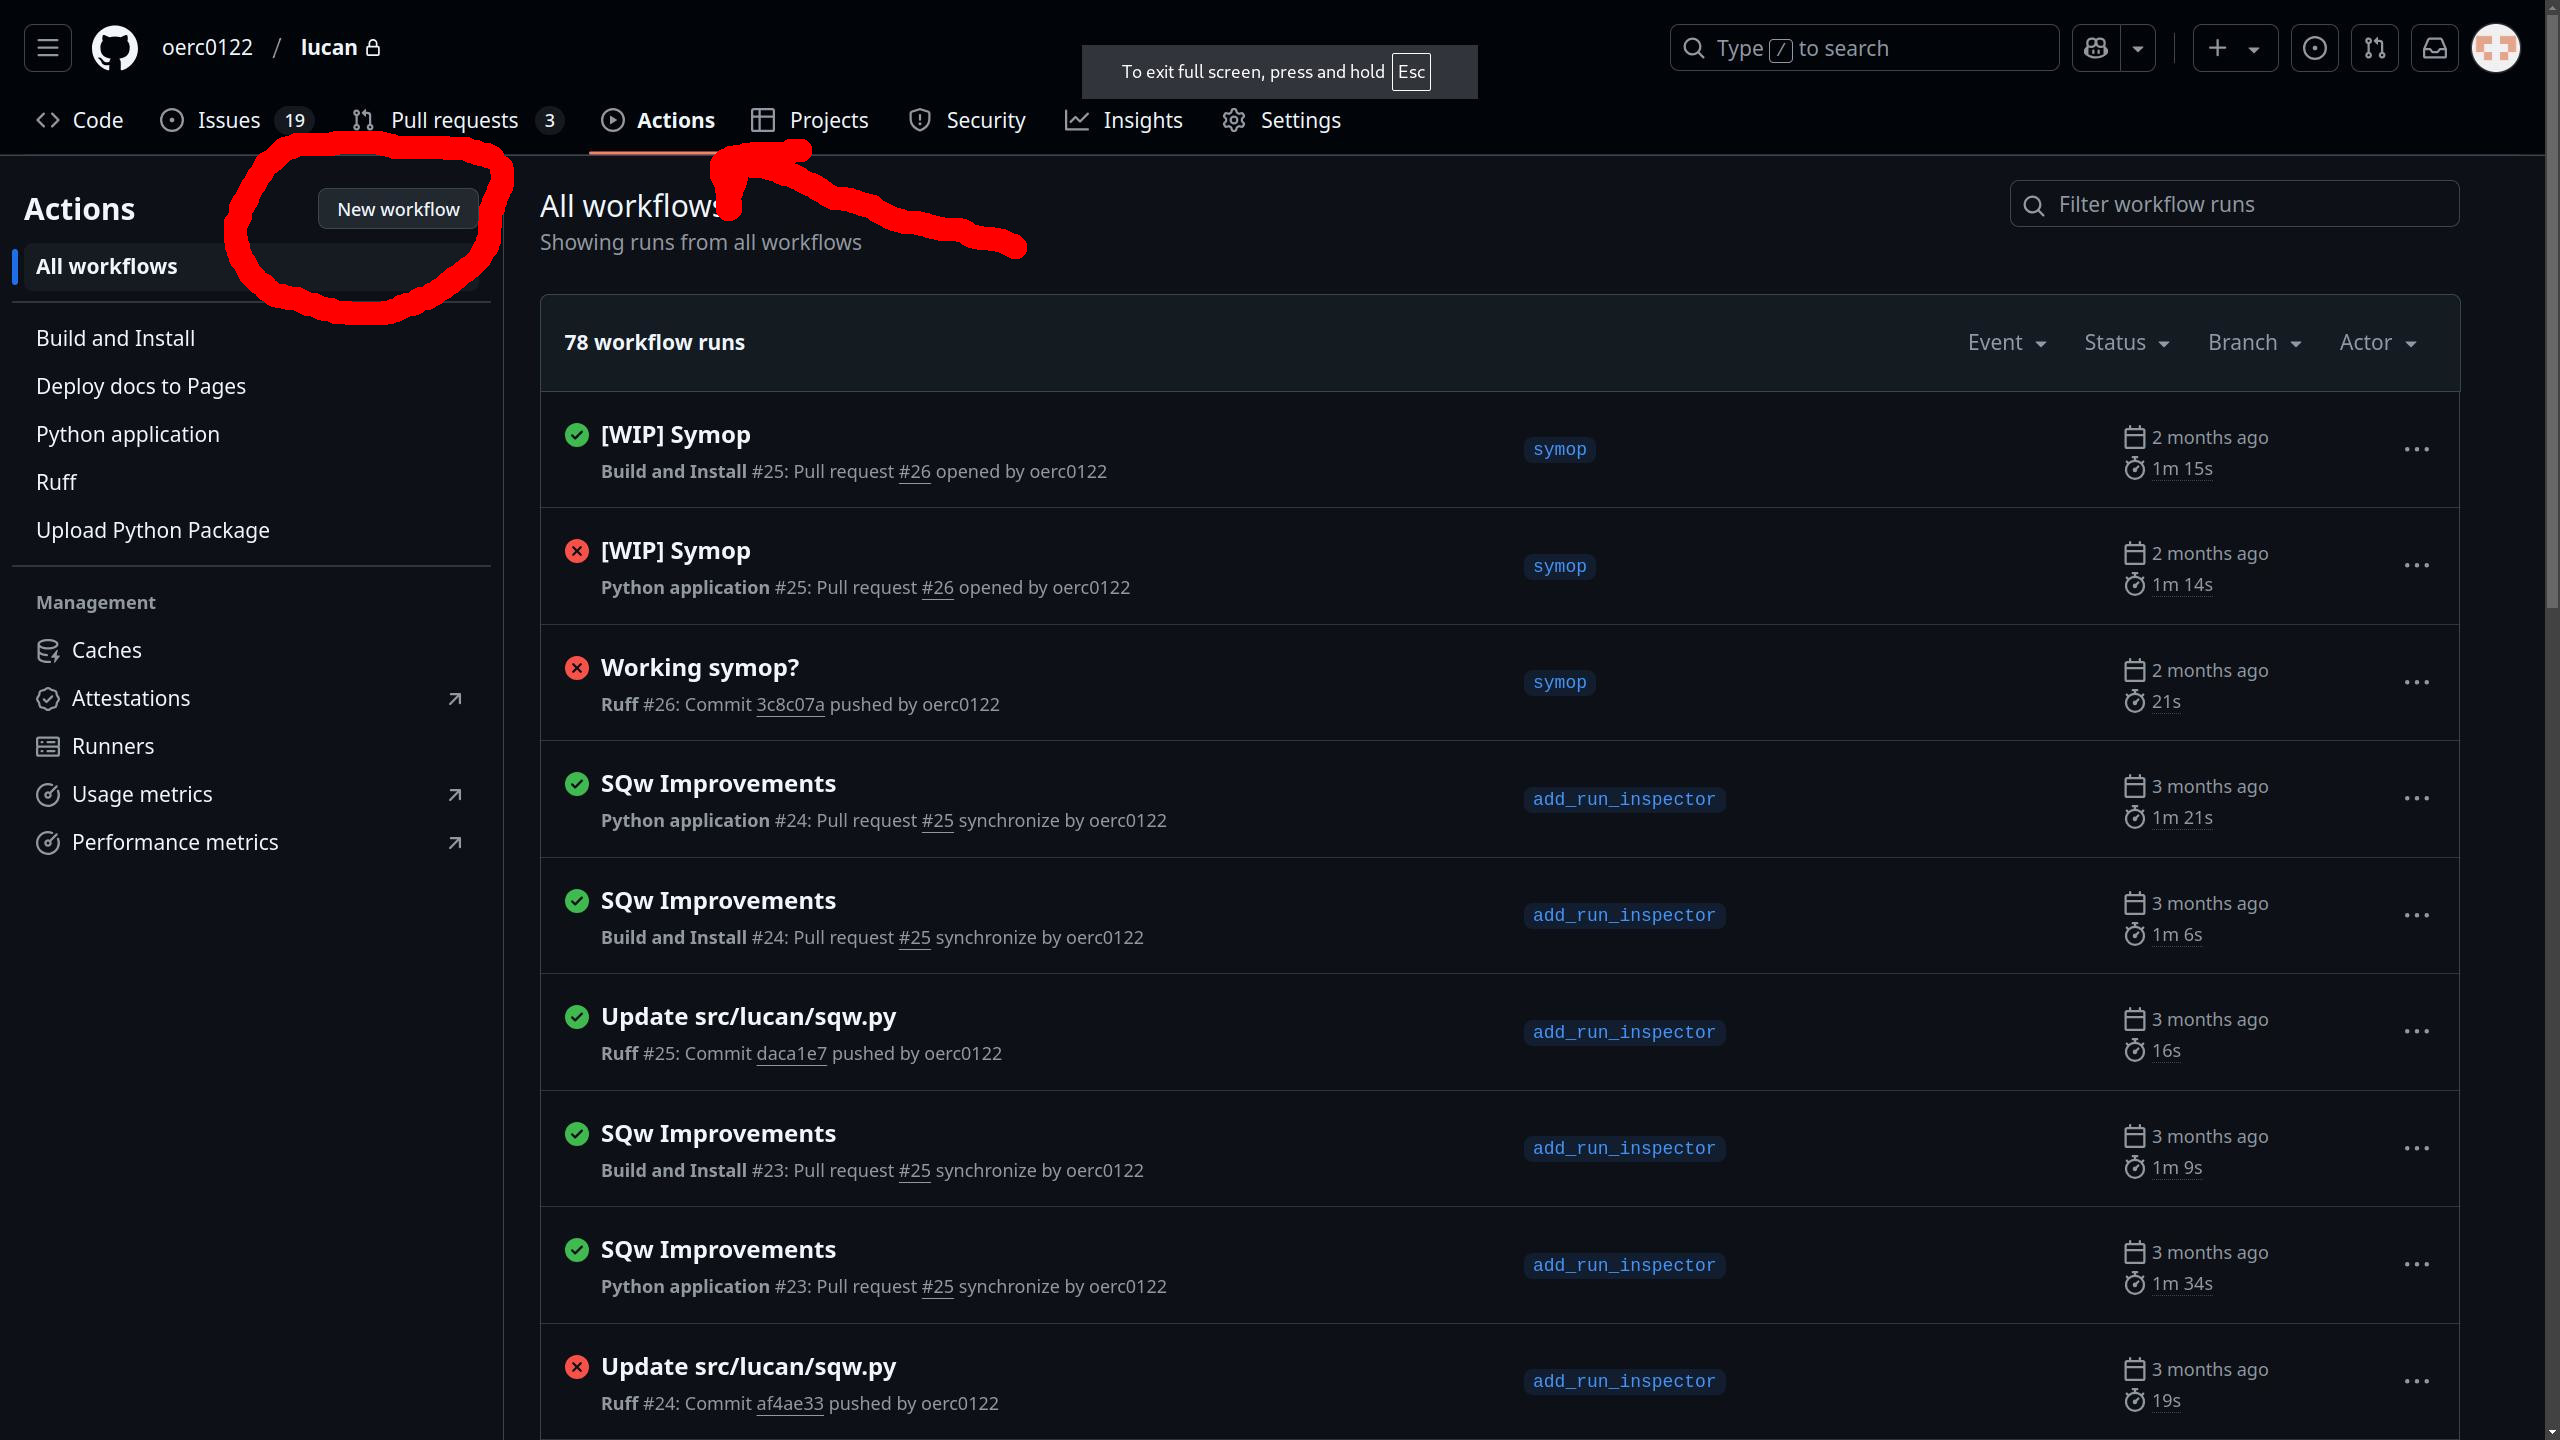
\includegraphics[width=0.9\textwidth]{findingmarket.jpg}
        \end{center}
    }
    \only<2-> {
        \begin{center}
            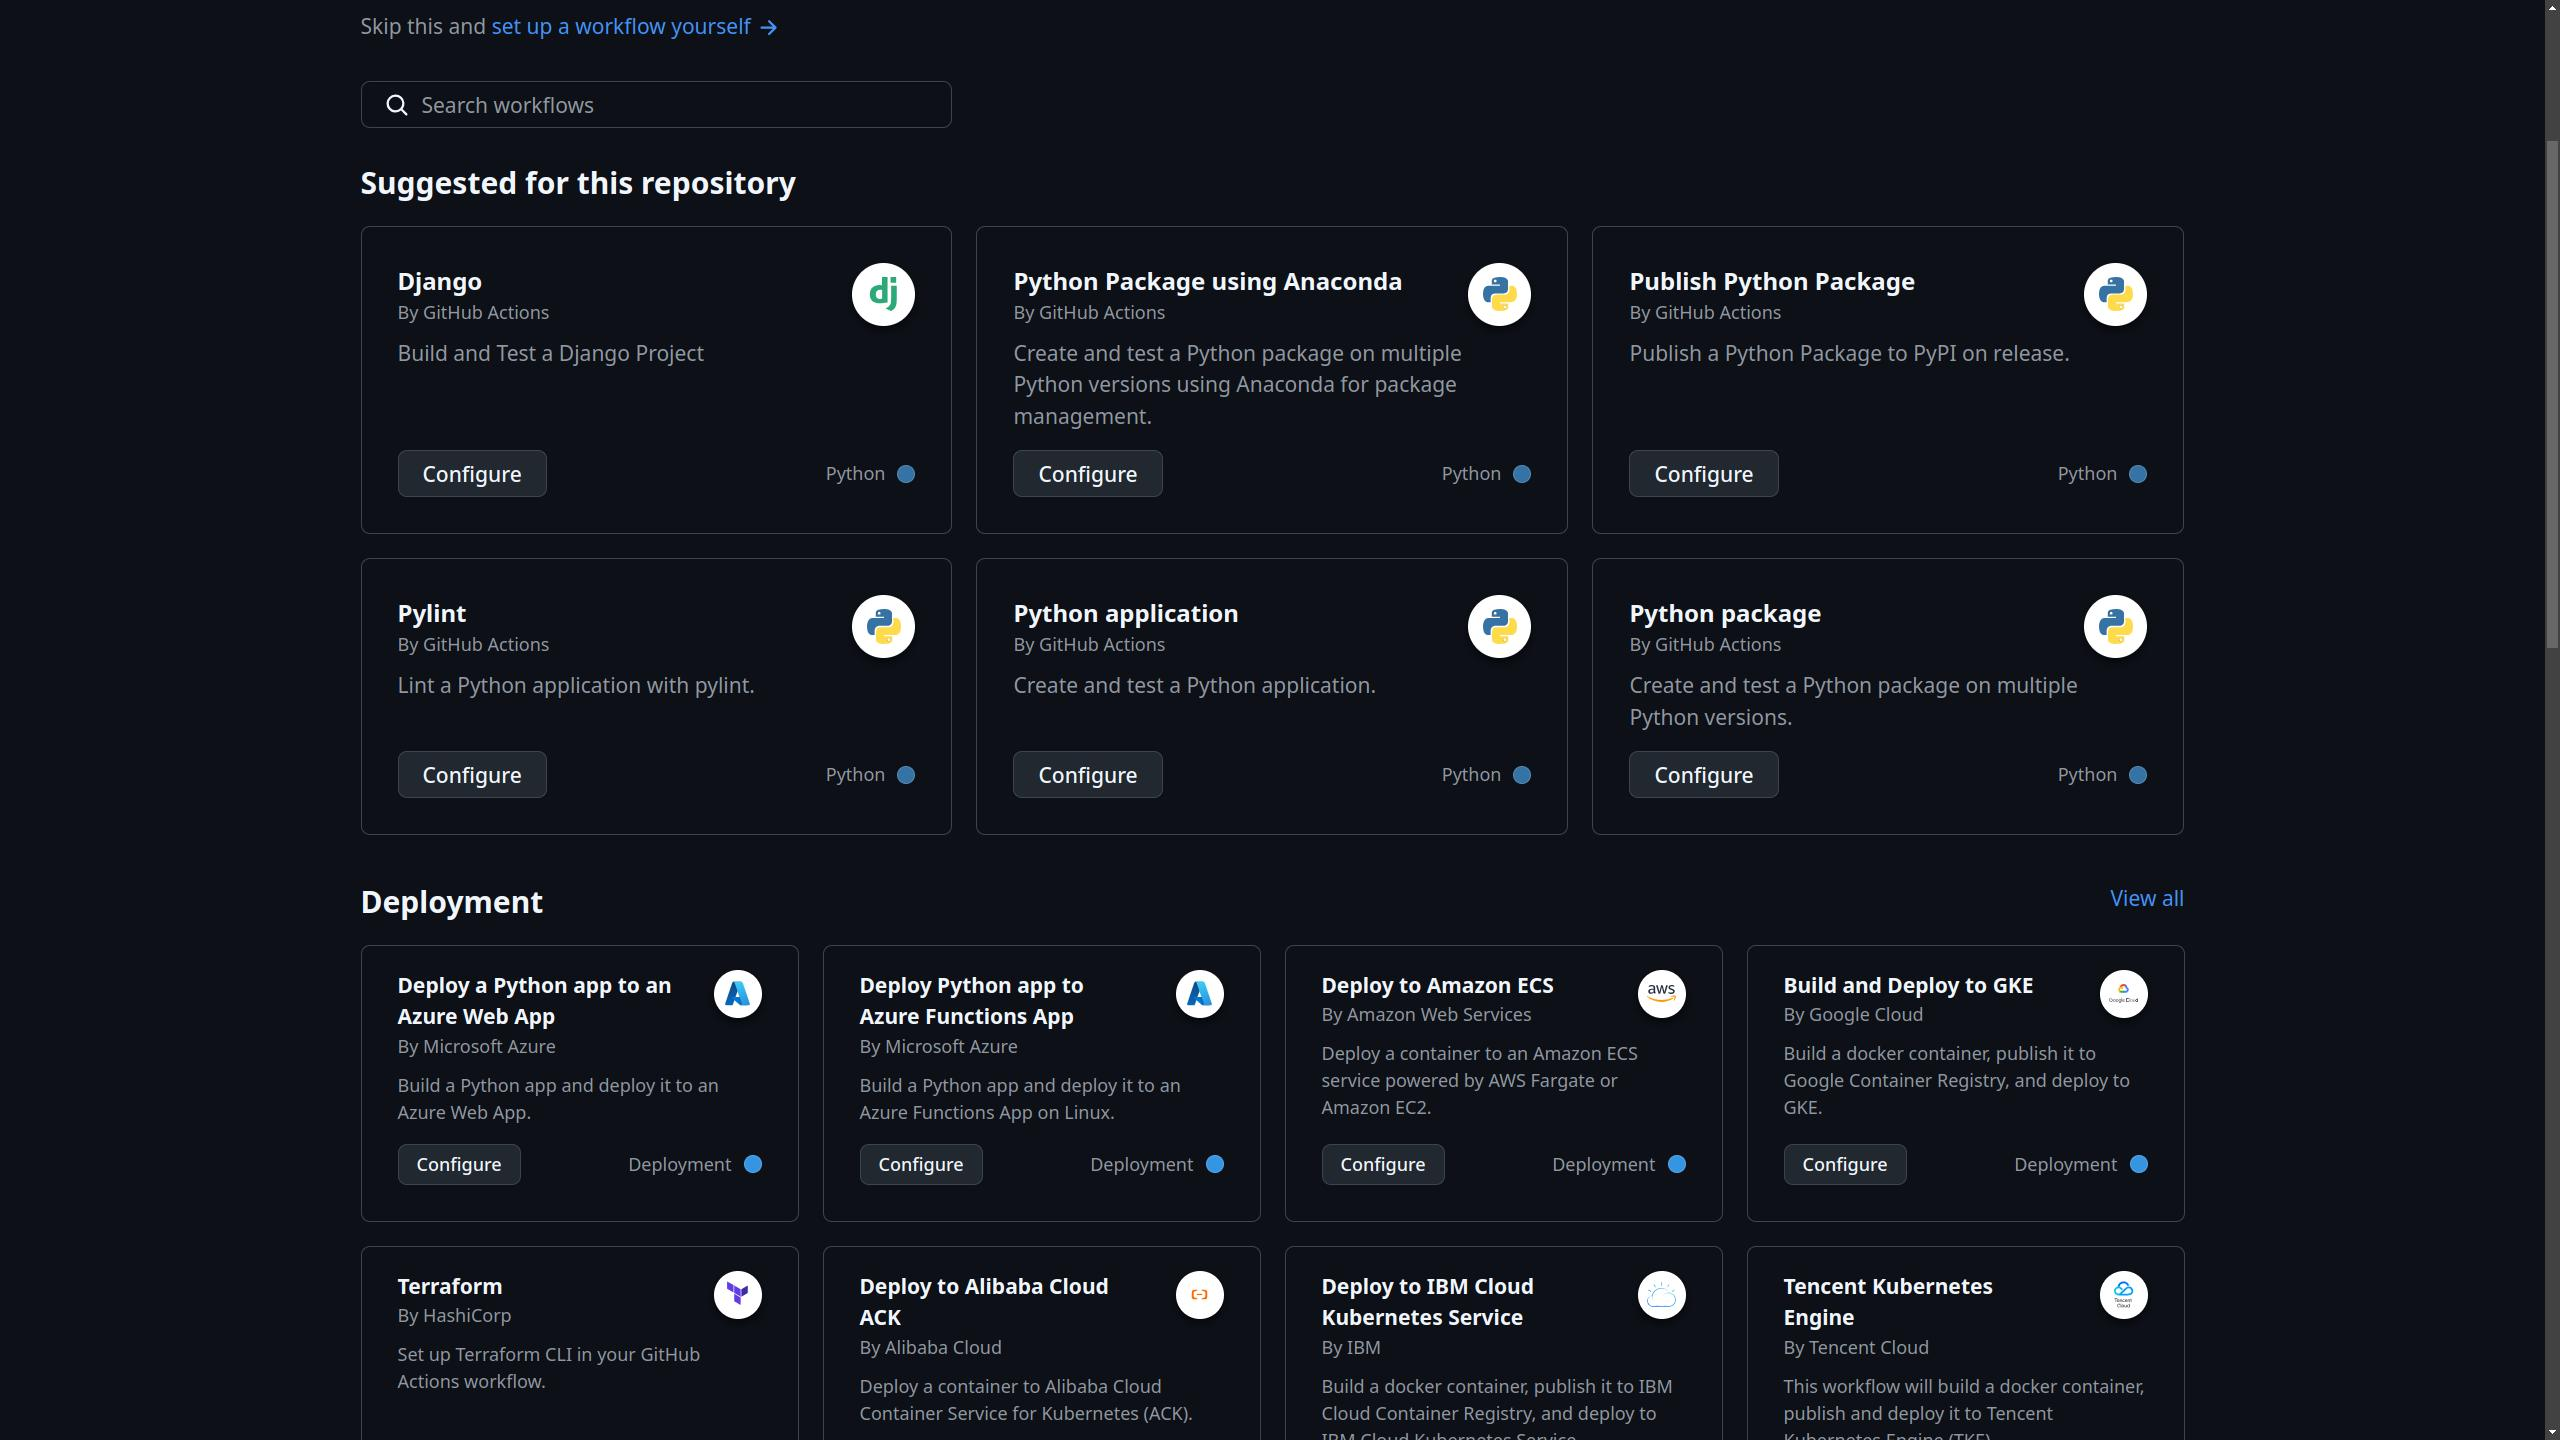
\includegraphics[width=0.9\textwidth]{exampleactions.jpg}
        \end{center}
    }
\end{frame}

\begin{frame}{Documentation in Action(s)}
    \begin{itemize}[<+->]
        \item{}But what about all the docs we've written?
        \item{}I don't want to host a website (but you can)!
        \item{}GitHub provides ``GitHub pages''; sites for projects.
        \item{}These can point to a branch or be managed by actions.
    \end{itemize}

    \only<3-> {
        \begin{center}
            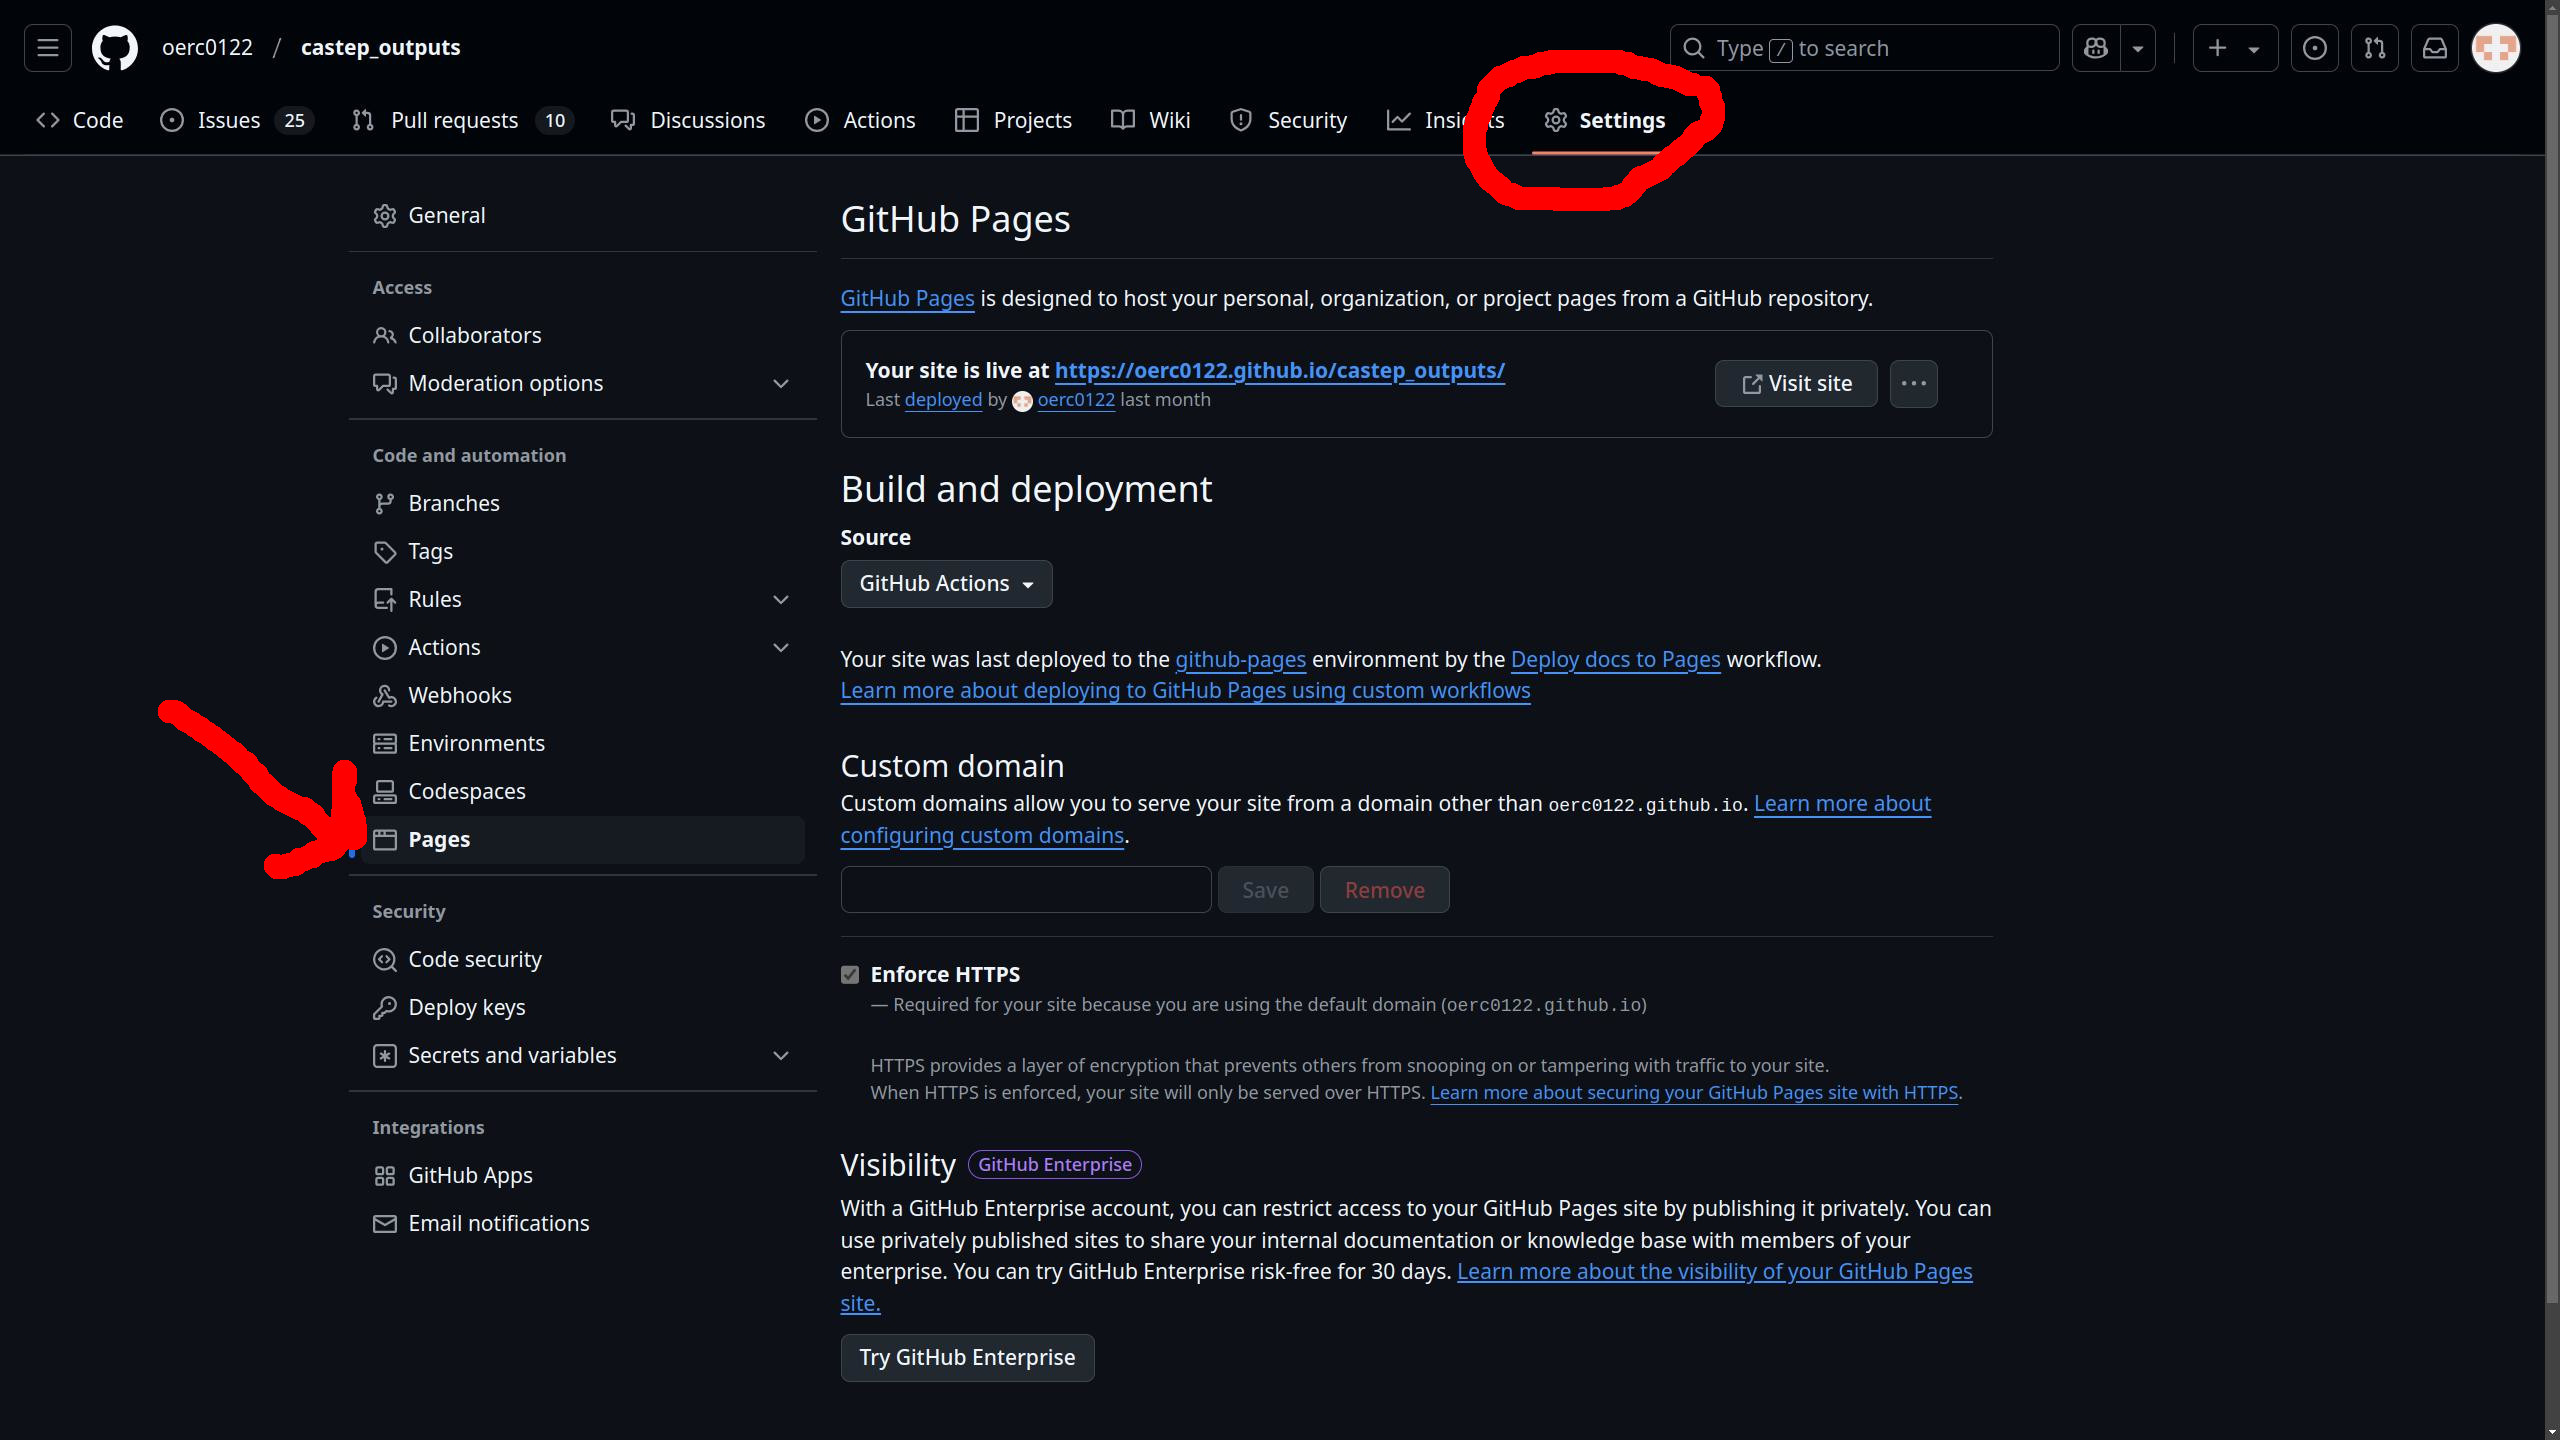
\includegraphics[width=0.9\textwidth]{ghpages.jpg}
        \end{center}
    }
\end{frame}

\begin{frame}{Documentation in Actions(s)}
    \begin{itemize}[<+->]
        \item{}So let's give it a go!
        \item{}Go to the marketplace and find an action doing (almost) what we want.\\ \tiny{Static Pages.}
        \item{}Add a bit of script to make it do (exactly) what we want.\\
        \tiny{Build the docs and upload those.}
        \item{}Run it!
        \item{}Go to \kw{https://<username>.github.io/polysolve}!
    \end{itemize}

    \only<1>{
        \begin{center}
            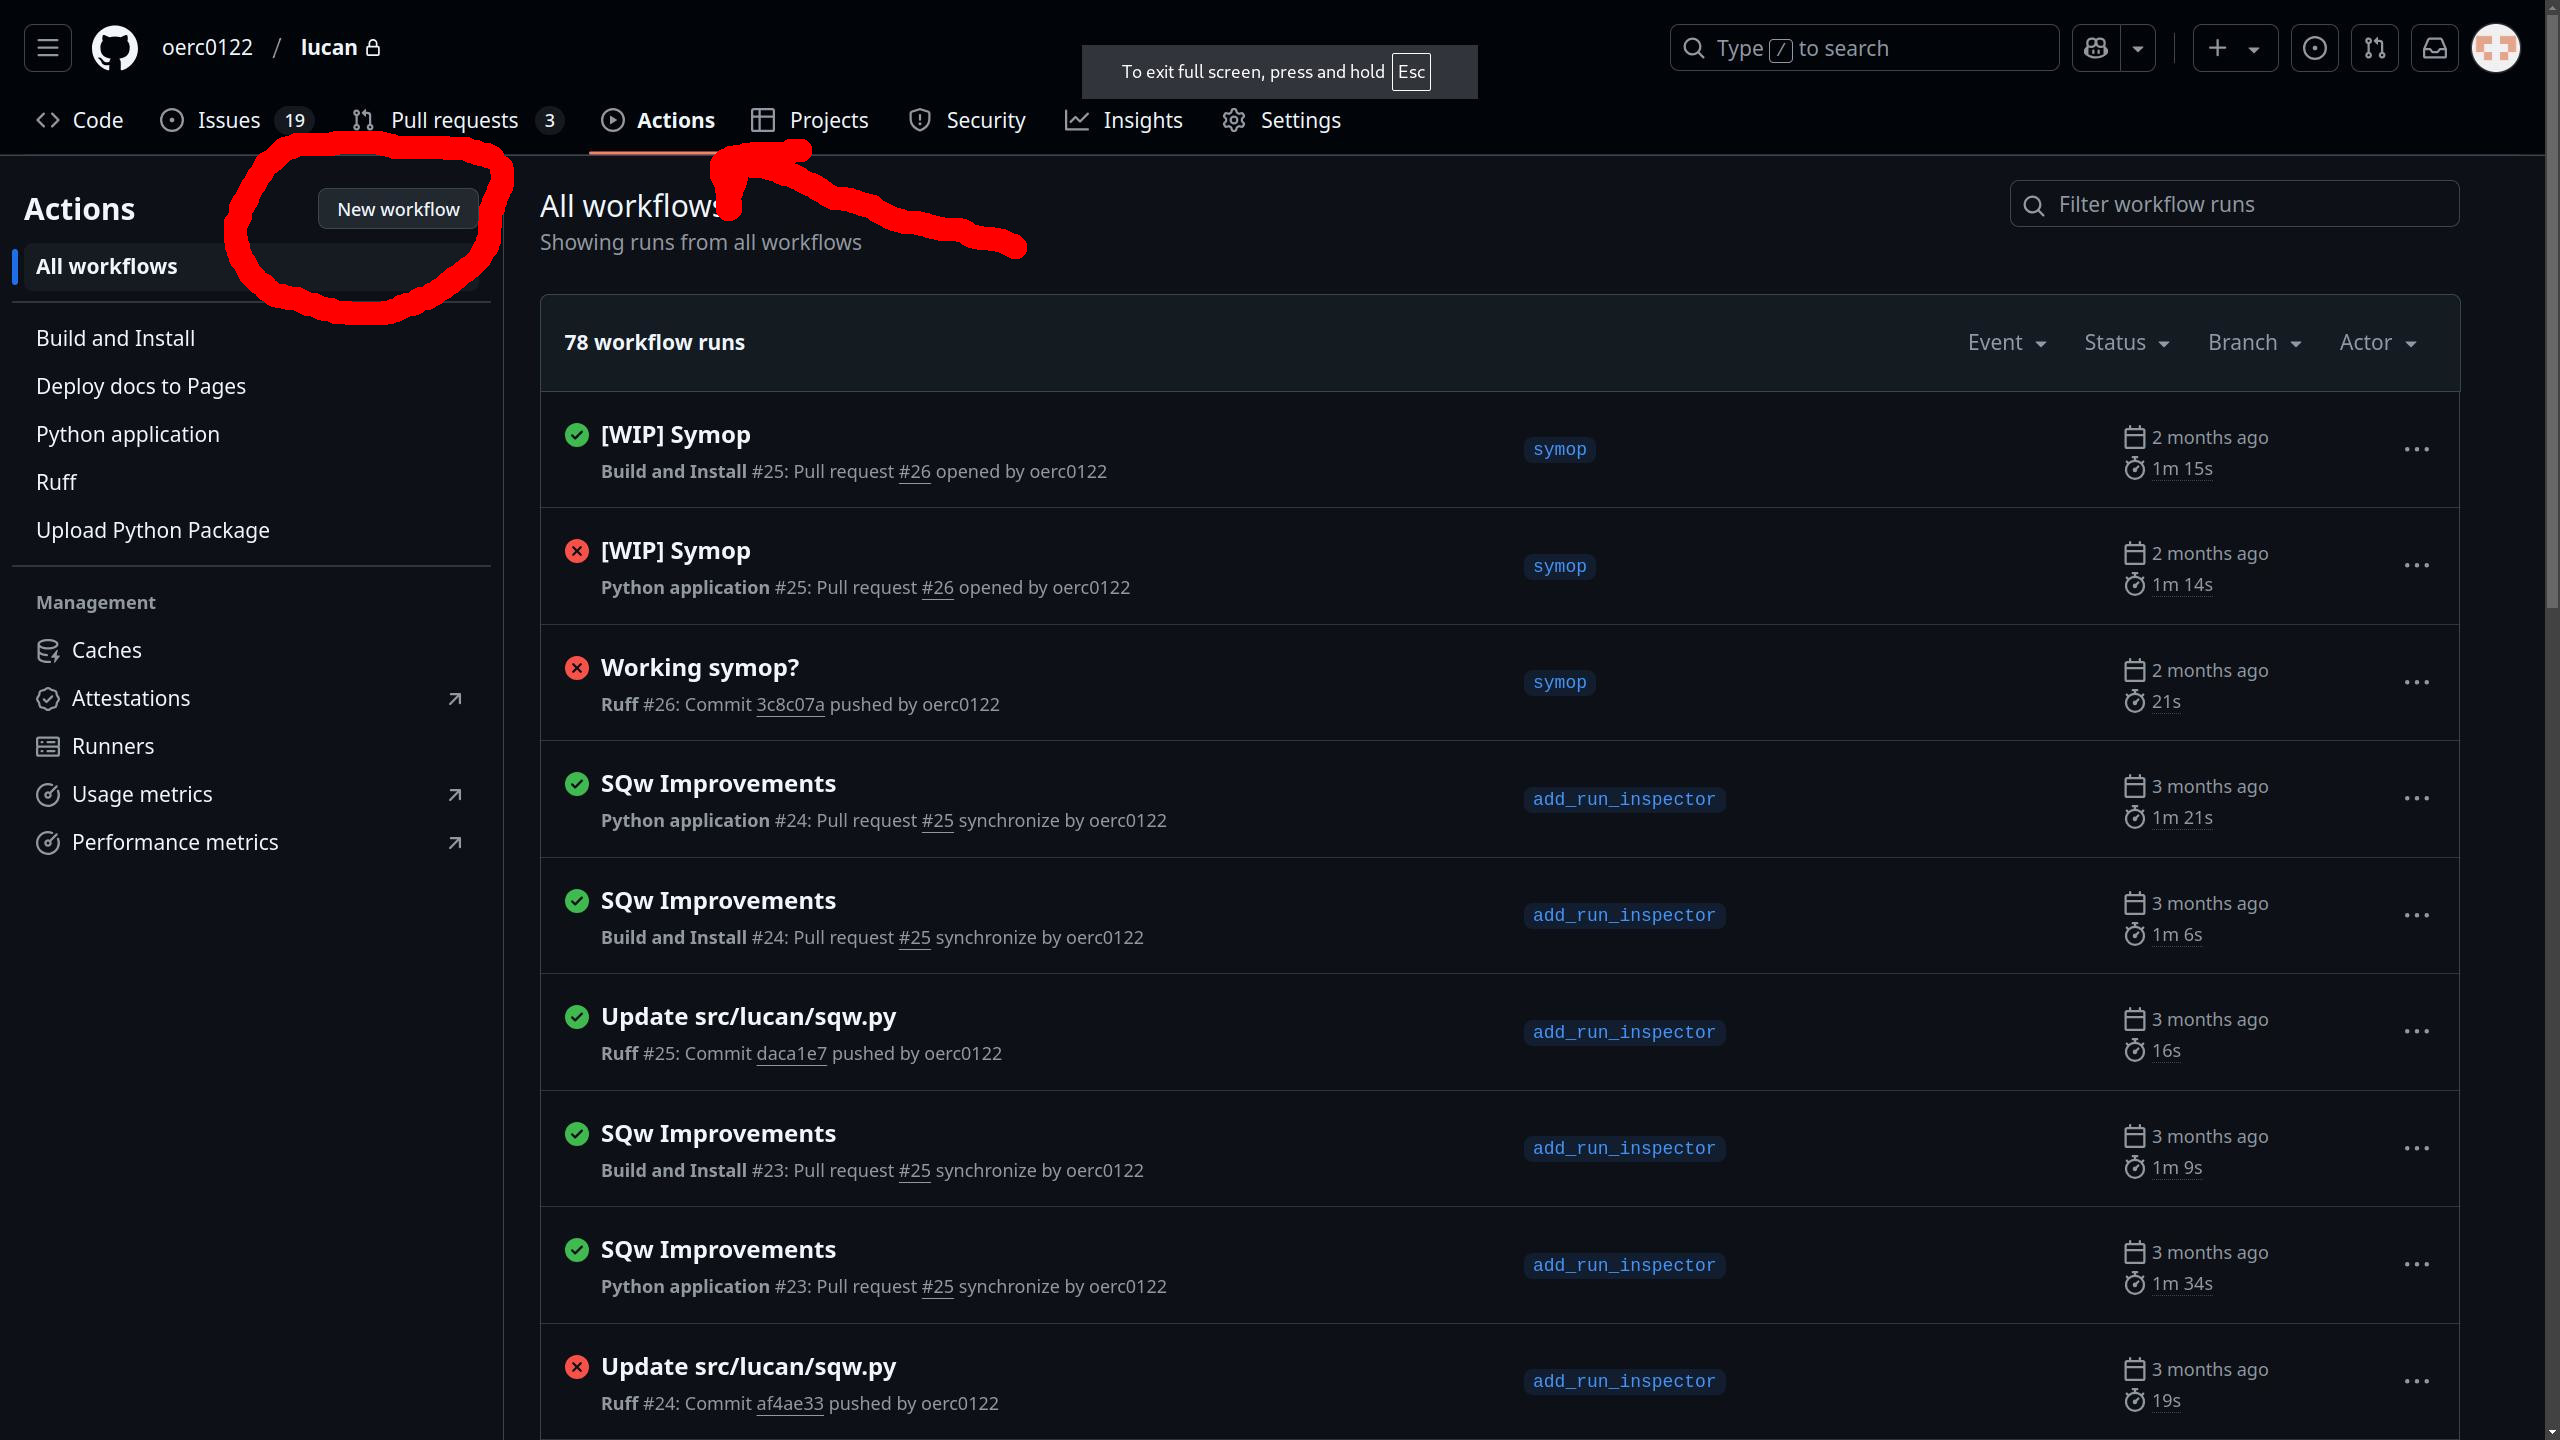
\includegraphics[width=0.9\textwidth]{findingmarket.jpg}
        \end{center}
    }
    \only<2>{
        \begin{center}
            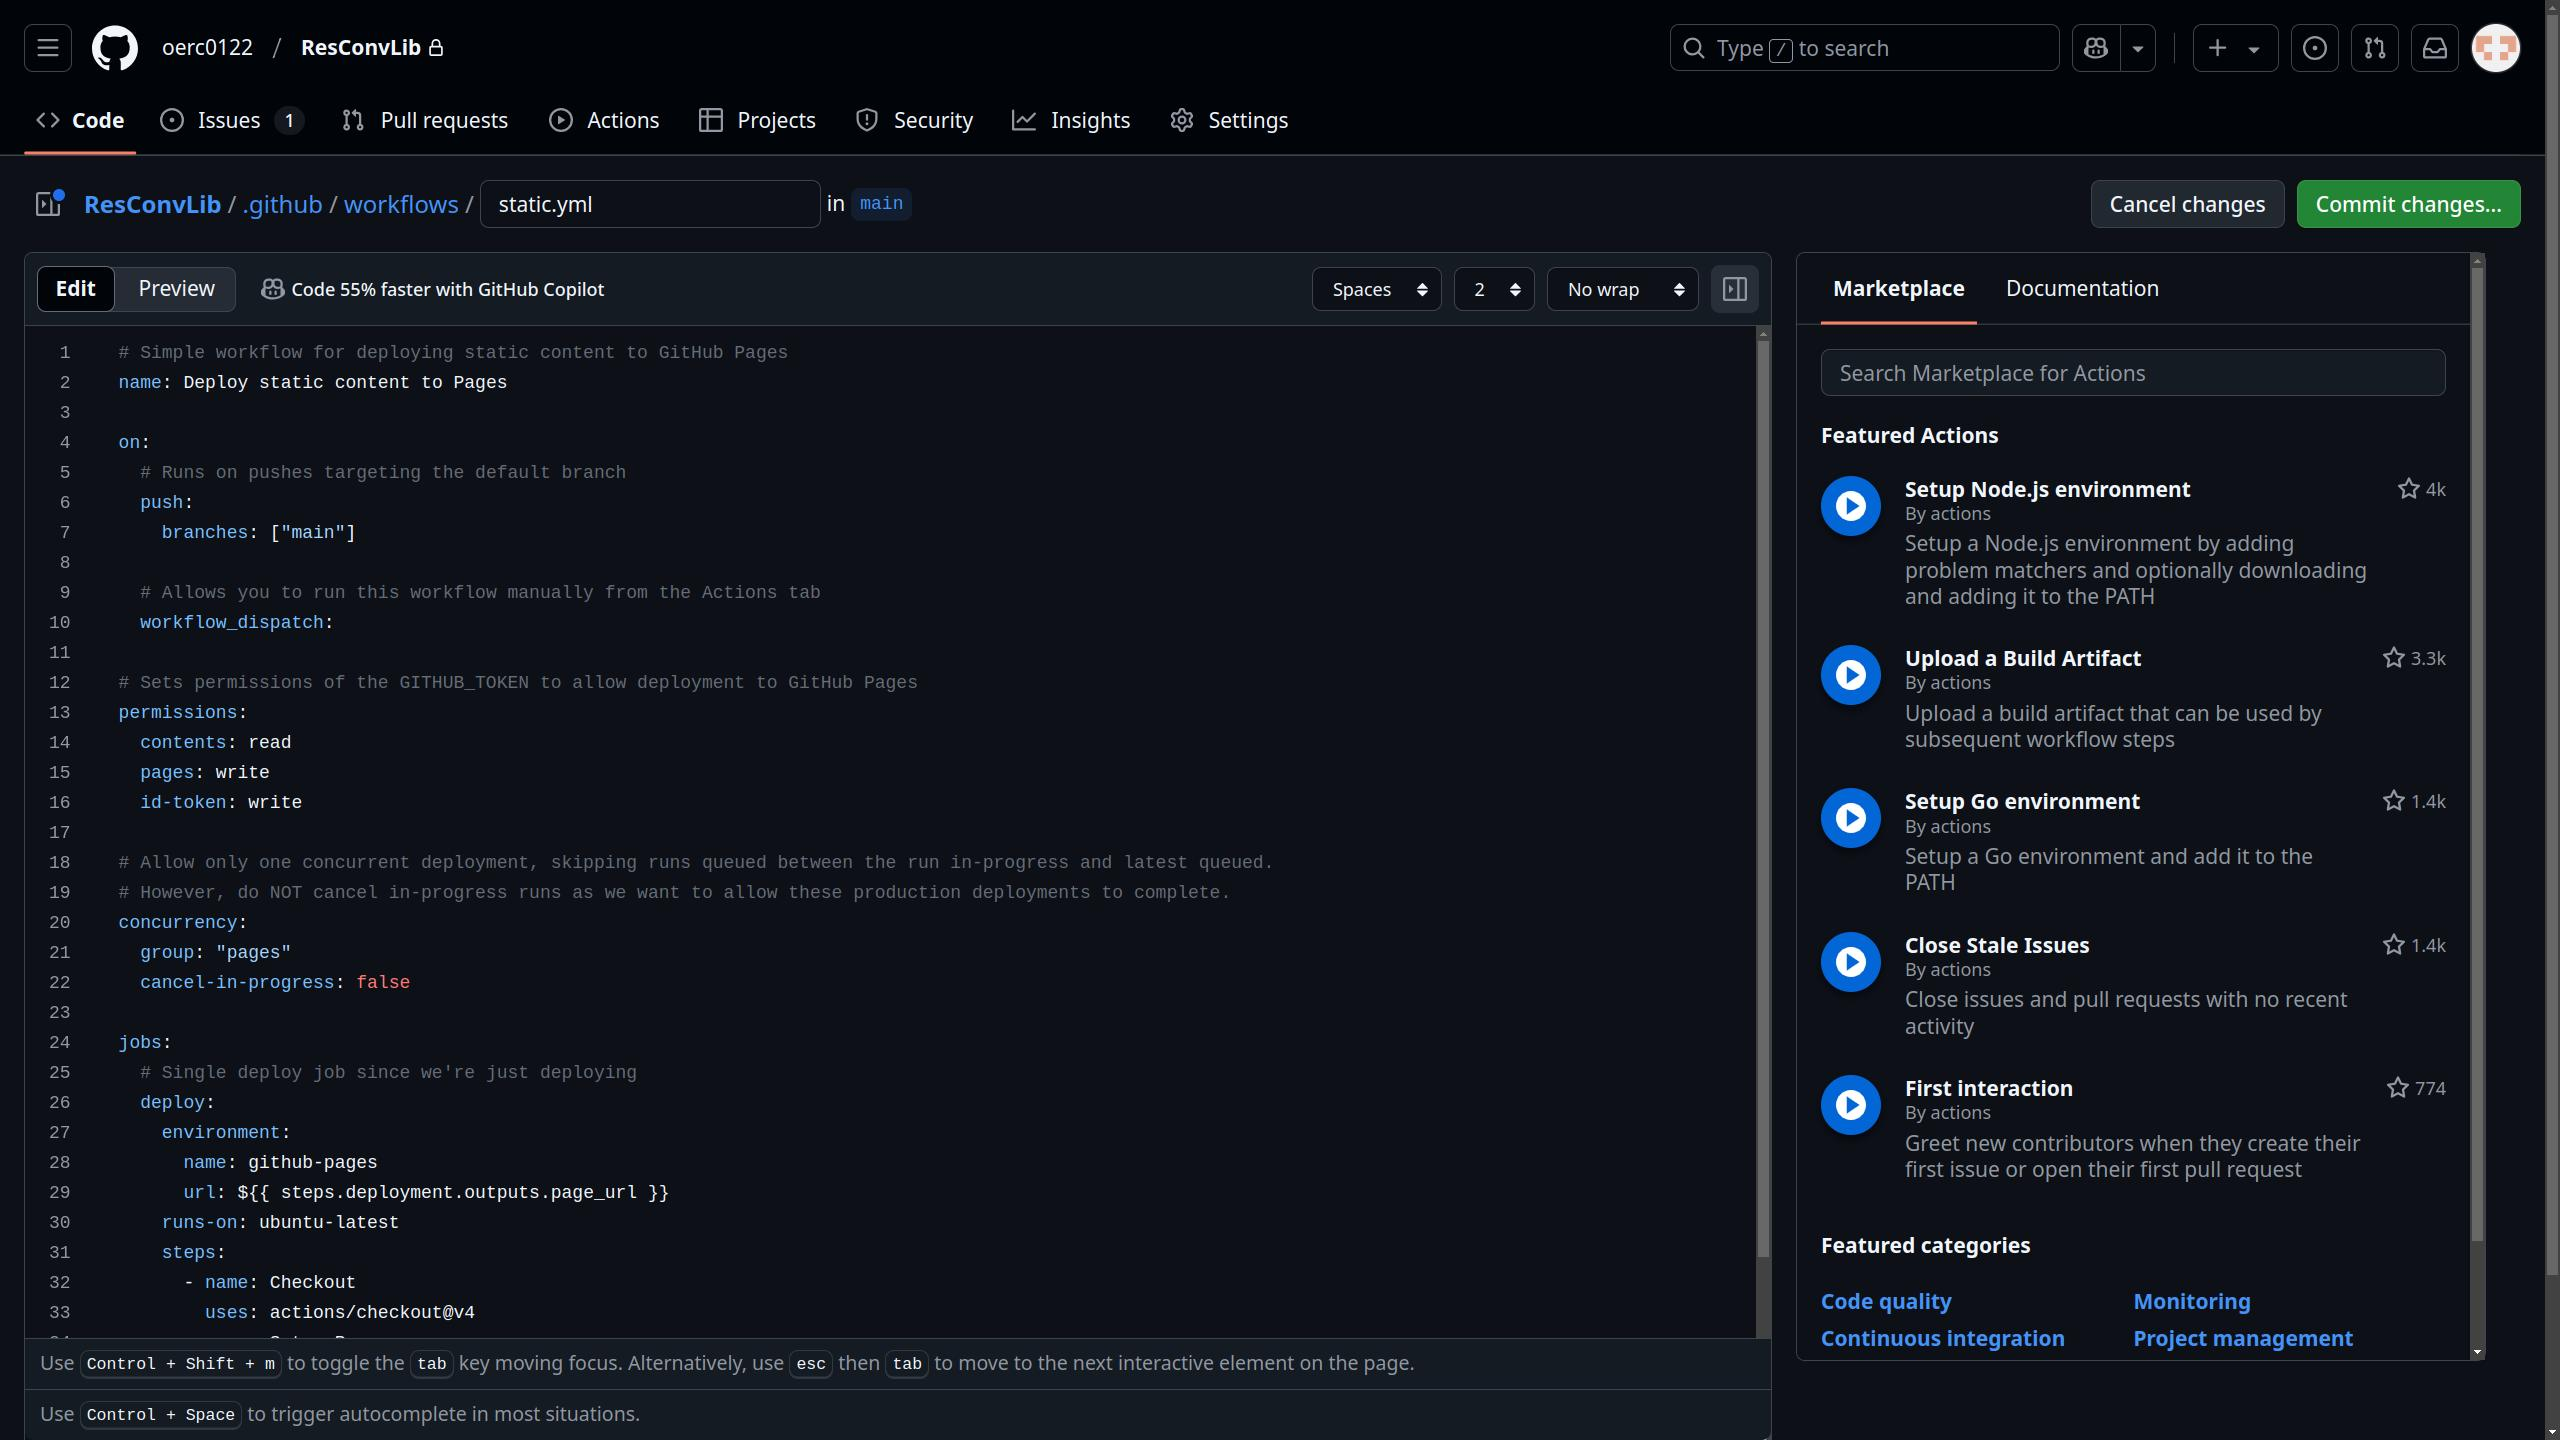
\includegraphics[width=0.9\textwidth]{original-action.jpg}
        \end{center}
    }
    \only<3>{
        \begin{center}
            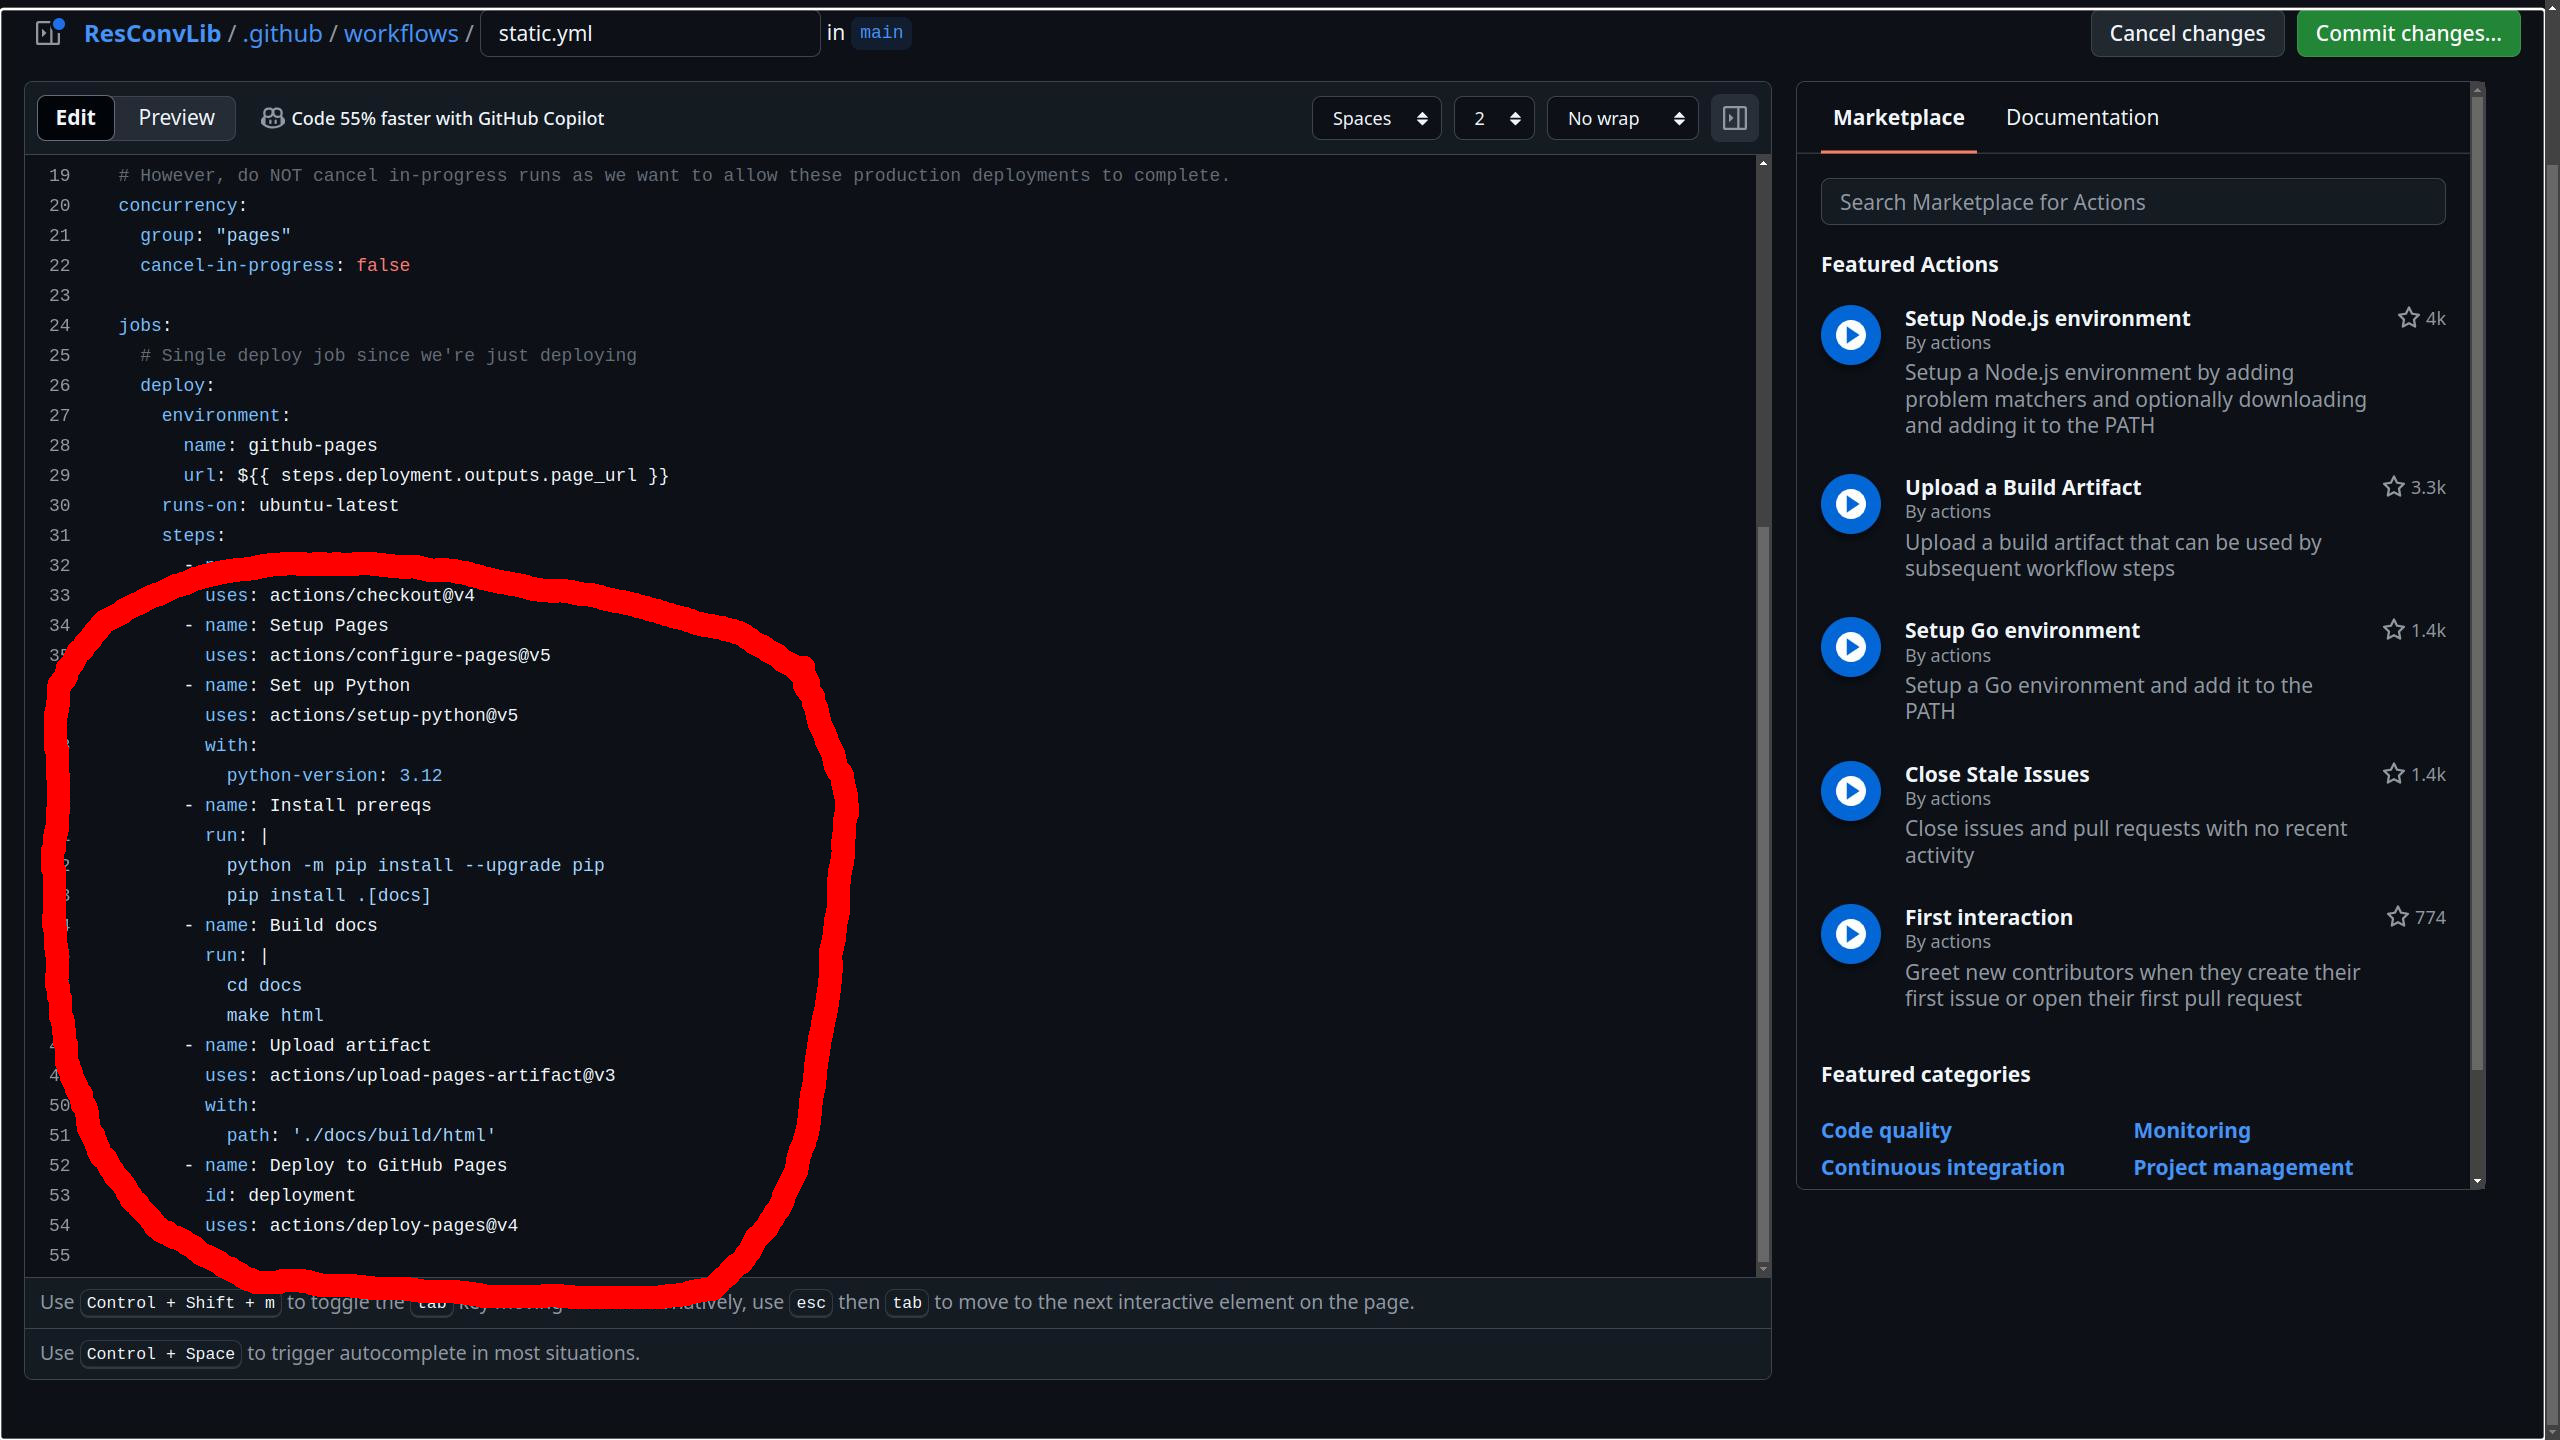
\includegraphics[width=0.9\textwidth]{modified-action.jpg}
        \end{center}
    }
    \only<4>{
        \begin{center}
            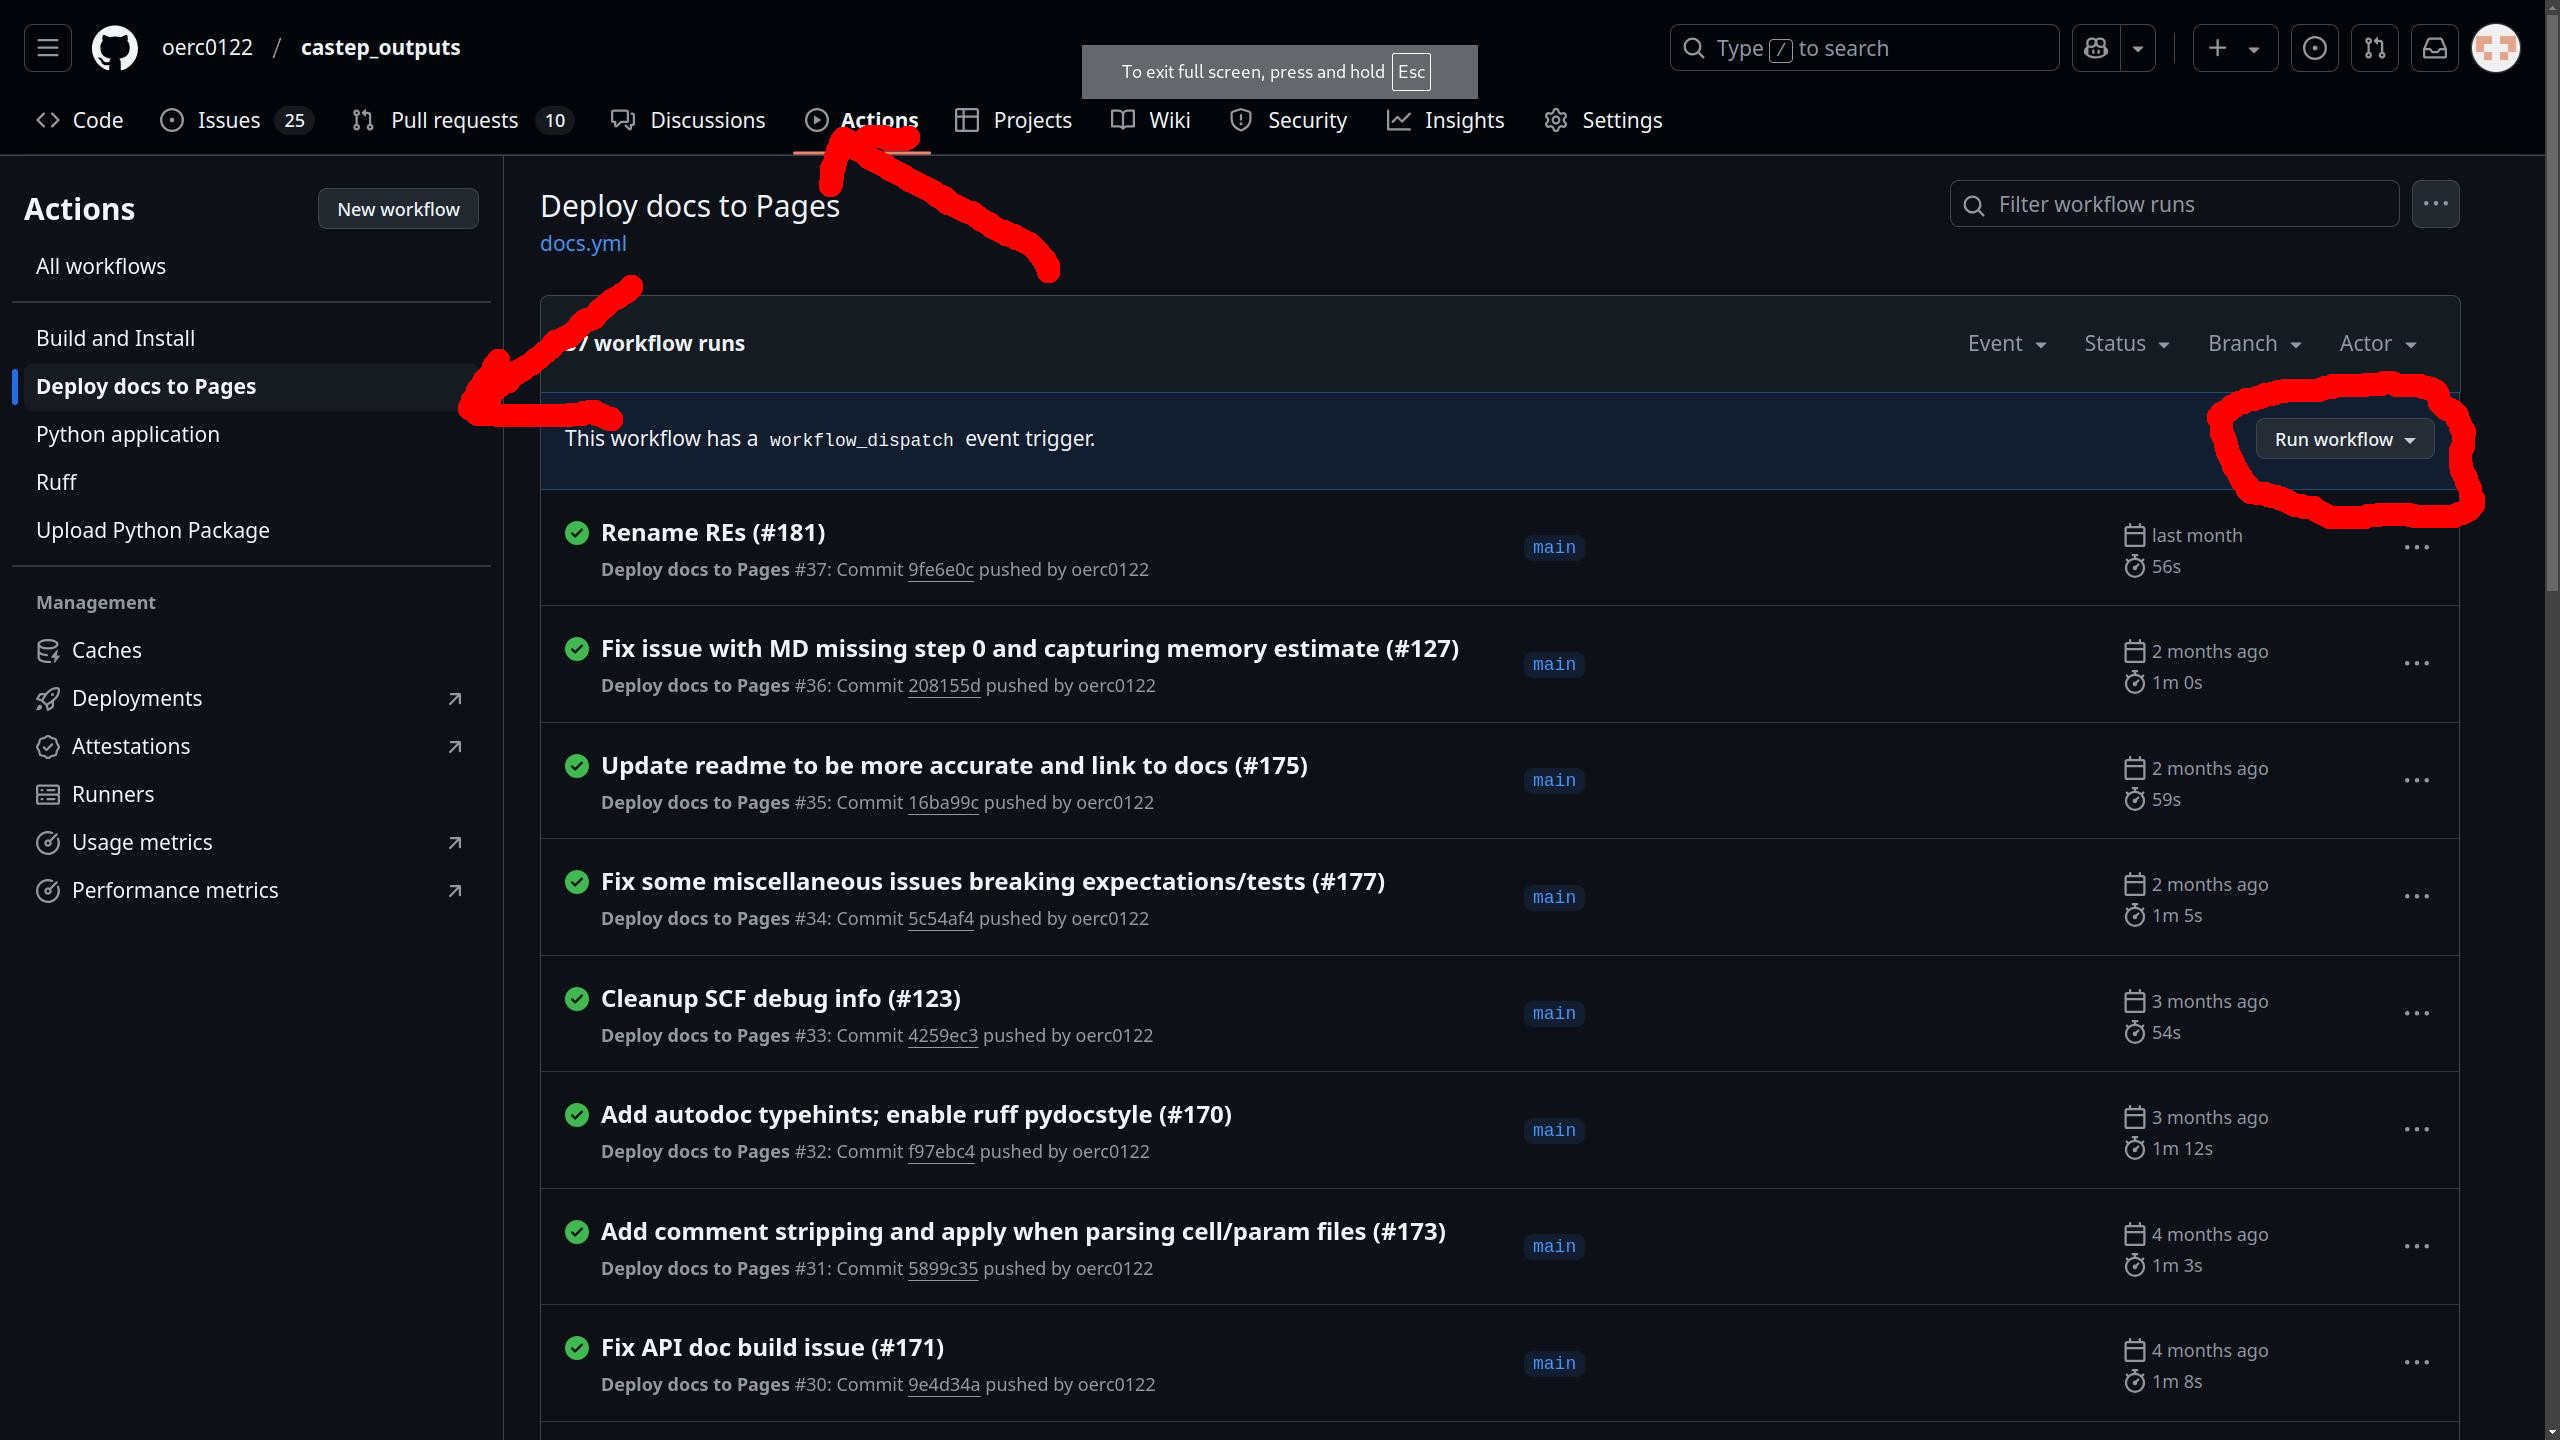
\includegraphics[width=0.9\textwidth]{manual-workflow.jpg}
        \end{center}
    }
\end{frame}

\section{Bonus}

\subsection{Attribution}

\begin{frame}{CITATION.cff}
    \begin{itemize}[<+->]
        \item{}Ok, so you've written the best project ever.
        \item{}At what point does the fame and glory start rolling in?
        \item{}Until people know how great you are that's not going to happen.
        \item{}\filet{CITATION.cff} is a standard format for code attribution.
        \item{}\url{https://citation-file-format.github.io/}
    \end{itemize}

    \only<4-5>{
        \lstinputlisting[basicstyle=\tiny]{CITATION.cff}
    }
    \only<6>{
        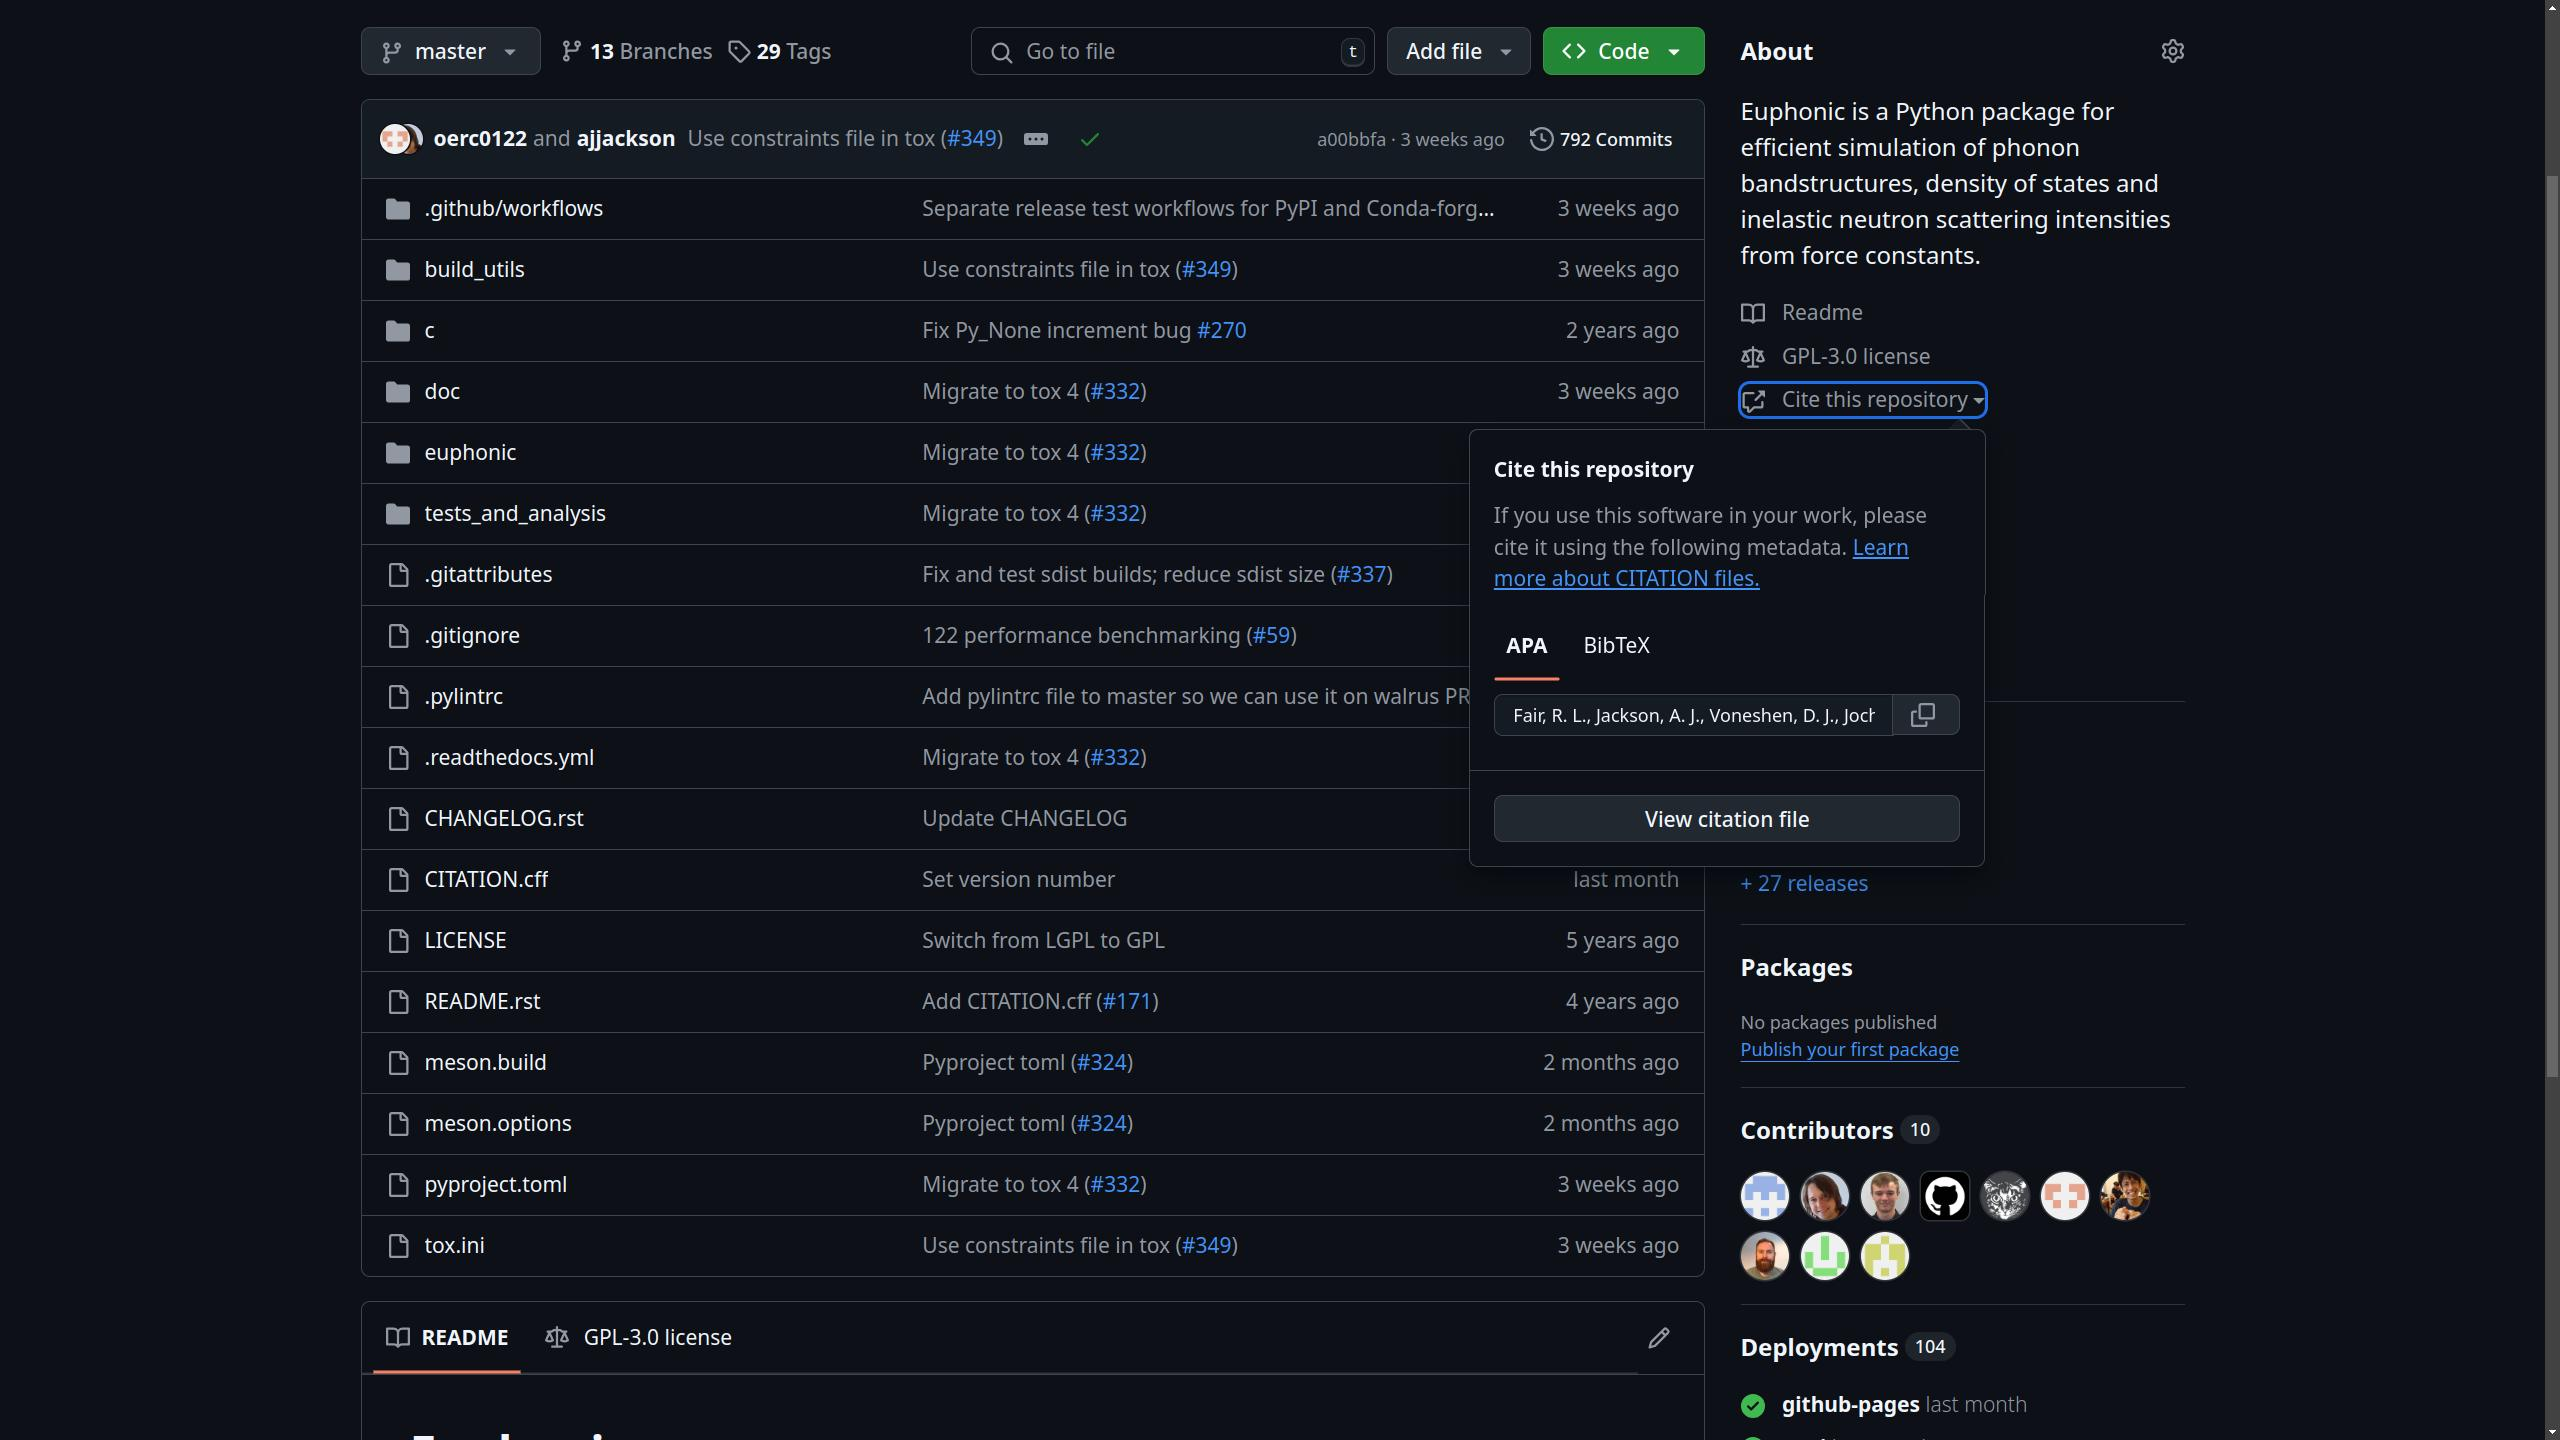
\includegraphics[width=0.9\textwidth]{CITATION.jpg}
    }
\end{frame}

\begin{frame}{DOIs}
    \begin{itemize}[<+->]
        \item{}Going a step further than just adding the citation file.
        \item{}Mint a DOI for a version of the software allowing it to be cited.
    \end{itemize}
\end{frame}

\begin{frame}{Extra tools}
    \begin{itemize}[<+->]
        \item{}Remember we mentioned an IDE easlier in the talk?
        \item{}An IDE is just one of many tools which can be helpful in development.
        \begin{itemize}
            \item{}IDE -- Specialised editor to make development easier 
            \begin{itemize}
                \item<.->{} (\cmd{VSCode}, \cmd{Spyder}).
            \end{itemize}
            \item{}Linting -- Checks for stylistic errors 
            \begin{itemize}
                \item<.->{} (\cmd{ruff}, \cmd{flake8}, \cmd{pylint})
            \end{itemize}
            \item{}Type checking -- Checks for passing the wrong data through 
            \begin{itemize}
                \item<.->(\cmd{mypy}, \cmd{pydantic}, \cmd{beartype})
            \end{itemize}
        \end{itemize}
    \end{itemize}
\end{frame}

\begin{frame}[fragile]{Ruff times}
    \begin{itemize}[<+->]
        \item{}Ruff\footnote{\url{https://docs.astral.sh/ruff/}} is a tool to encourage (enforce) code standards.
        \item{}Modern replacement for half a dozen prior tools.
        \item{}Flags violations of code standards.
        \item{}Also handles formatting code
        \item{}Customisable through \filet{pyproject.toml}
    \end{itemize}

    \begin{onlyenv}<1>
        \begin{block}{Adding it in}
            \begin{lstlisting}[basicstyle=\scriptsize]
[project.optional-dependencies]
docs = ["sphinx",
        "sphinx-rtd-theme", 
        "sphinx_autodoc_typehints"]
test = ["pytest"]
lint = ["ruff=0.8.0"]
            \end{lstlisting}
        \end{block}
    \end{onlyenv}

    \begin{onlyenv}<3>
        \begin{block}{Try it out!}
            \cmd{ruff check}
        \end{block}
     \end{onlyenv}
     
    \begin{onlyenv}<4>
        \begin{block}{Try it out!}
            \cmd{ruff format}
        \end{block}
    \end{onlyenv}

    \begin{onlyenv}<5>
        \lstinputlisting[basicstyle=\scriptsize,linerange={13-19,38}]{ruff-config.toml}
    \end{onlyenv}

    \begin{onlyenv}<6>
        \lstinputlisting[basicstyle=\scriptsize,linerange={1-4,50-52}]{ruff-config.toml}
    \end{onlyenv}

\end{frame}

\begin{frame}{Ruff times\footnote[]{\filet{lint.yml}}}
    \lstinputlisting[basicstyle=\scriptsize]{lint.yml}
\end{frame}

\begin{frame}{cookiecutter}
    \begin{itemize}[<+->]
        \item{}Possible to take out some of the boilerplate of setup.
        \item{}\url{cookiecutter.io} is a set of pre-configured project folders.
        \item{}Modules for many languages (including Python)
    \end{itemize}
\end{frame}

\begin{frame}{Checklist}
    \begin{description}
        \item[$\square$]Sensible names
        \item[$\square$]On GitHub
        \item[$\square$]Project layout
        \begin{description}
            \item[$\square$]\filet{__init__.py}
            \item[$\square$]\filet{pyproject.toml}
        \end{description}
        \item[$\square$] Documentation
        \begin{description}
            \item[$\square$]Docstrings
            \item[$\square$]Doctests
            \item[$\square$]Typehints
            \item[$\square$]\kw{sphinx-quickstart}
            \item[$\square$]\kw{sphinx-apidoc}
        \end{description}
        \item[$\square$]Tests
        \item[$\square$]CI/CD
        \begin{description}
            \item[$\square$]Automated testing
            \item[$\square$]Automatic documentation
        \end{description}
        \item[$\square$]\filet{CITATION.cff}
    \end{description}
\end{frame}


\end{document}